\documentclass[10pt]{article}
\usepackage{lecture-report}
\usepackage{listings}
\usepackage{amsmath}

% Pseudocode boxes in the house accent-bar style
\lstdefinestyle{house}{
  basicstyle=\ttfamily\footnotesize,
  keywordstyle=\bfseries,
  commentstyle=\color{slate}\itshape,
  backgroundcolor=\color{graypale},
  frame=l, framerule=2.2pt, rulecolor=\color{tealdark},
  xleftmargin=3.2mm, framexleftmargin=2.6mm,
  aboveskip=7pt, belowskip=7pt,
  columns=fullflexible, keepspaces=true,
  language=Python, showstringspaces=false,
  literate={–}{--}1,
}
\lstset{style=house}

\reporthead{DRAWMAHA SOLVER PROJECT}{How poker solvers are trained}

\begin{document}
\reporttitle{How Poker Solvers Are Trained}%
{A field guide to the ML behind equilibrium poker --- written to start the first Drawmaha solver}%
{research synthesis of 70 sources \,\textperiodcentered\, August 28, 2026}

% ---------------------------------------------------------------- abstract
\textbf{Abstract.} This survey explains how machine-learning poker solvers are actually built and trained: what ``solving'' a poker game means, why the standard applied-RL toolkit (reward functions, actor--critic, self-play) fails at it, and what the poker-AI community built instead --- the counterfactual-regret family, its neural descendants, the search-plus-value-network lineage, and the modern RL methods that fix self-play's cycling. Every method is presented intuition-first, with its tradeoffs and its meaning for one concrete project: building the first solver for heads-up pot-limit Drawmaha, a split-pot draw/Omaha hybrid with 2{,}598{,}960 possible starting hands and no prior solver, bot, or academic mention as of August 2026. It closes with the full checklist of design decisions the project will face. Synthesized from an eight-lane literature sweep (about 70 verified sources); the cited originals remain ground truth.

\begin{tldr}
\begin{itemize}
\item ``Solving'' means computing a \textbf{Nash equilibrium} --- a strategy so balanced that even an opponent who knows it exactly cannot beat it. Its distance-from-perfect is a measurable number, \textbf{exploitability}.
\item The entire field rests on one ten-line rule, \textbf{regret matching}, and one theorem: the \emph{average} of self-play strategies converges to equilibrium while the current strategy cycles forever. Deploy the average, never the last iterate.
\item \textbf{CFR} runs that rule at every decision point of the game tree; \textbf{MCCFR} samples the tree instead of walking it; \textbf{Deep CFR} replaces the regret tables with networks when the game no longer fits in memory. This is the project's spine.
\item Naive PPO-style self-play has \emph{no} equilibrium guarantee in poker --- the dynamics provably orbit instead of converging. Every working RL fix restores convergence by averaging, populations, or regularization.
\item Training loss means nothing here; the only honest progress meters are exploitability on small games and best-response probes plus variance-reduced head-to-head at full scale.
\item Drawmaha adds three specific complications --- a 2.6M-hand space, a draw round with a public draw count, and a split pot --- and the literature has a precedent for each; the split pot is the cheapest of the three.
\end{itemize}
\end{tldr}

\section{``Solving'' means unexploitable, and unexploitable is a number}\label{sec:solving}

\mkey{what solving means}Machine learning usually optimizes against a fixed target: a loss goes down, accuracy goes up. Poker has no fixed target. The quality of any strategy depends entirely on what the opponent does, and the opponent adapts. So the field's definition of ``solved'' is borrowed from game theory: a strategy pair is a \keyterm{Nash equilibrium}\mdef{Nash equilibrium}{a pair of strategies where neither player can gain by changing only their own} when neither player can improve by deviating unilaterally. \hlight{An equilibrium strategy is one you could publish --- an opponent who reads your exact strategy still cannot beat it in expectation.}

Three classical facts make this the right target for \emph{heads-up} poker, and they are worth internalizing before any algorithm:

\begin{enumerate}
\item \textbf{Two-player zero-sum is special.} Heads-up poker is \keyterm{zero-sum}\mdef{zero-sum}{whatever one player wins, the other loses; payoffs sum to a constant} --- every chip you win, the opponent loses. Von Neumann's minimax theorem says such games have a unique \emph{value} (the expected win rate of perfect play), and all equilibria achieve it. Better: equilibria are \emph{interchangeable} --- any equilibrium strategy of yours is safe against any strategy of theirs, guaranteeing at least the game value. This is exactly what fails with three or more players, which is why every guarantee in this survey is heads-up-only (Section~\ref{sec:checklist} returns to this).
\item \textbf{Equilibrium play must be random.} If you only bet when strong, your bets stop getting paid; if you never bluff, your checks get attacked. The equilibrium bluffs, calls, and value-bets with calibrated \emph{frequencies} --- it is a \keyterm{mixed strategy}\mdef{mixed strategy}{a probability distribution over actions, rather than one fixed action}. \pitfall{This single fact --- optimal play is deliberately stochastic --- is what breaks most standard RL machinery later in this survey}: greedy ``take the best action'' improvement has no fixed point to find.
\item \textbf{Distance from equilibrium is measurable.} Fix your strategy $\sigma$ and let a perfect adversary --- the \keyterm{best response}\mdef{best response}{the strategy maximizing EV against one known, fixed opponent strategy} --- extract the maximum from it. What it wins above the game value is your \keyterm{exploitability}\mdef{exploitability}{how much a perfect counter-strategy beats your strategy for; zero exactly at equilibrium}. Exploitability is the loss function of this entire field: every algorithm in this survey is judged by how fast it drives that number toward zero, and Section~\ref{sec:evaluation} is about how to measure it at each scale.
\end{enumerate}

\subsection*{The object being solved: a game tree with hidden cards}

\mkey{extensive form}Poker is played on a tree: chance nodes deal cards, decision nodes belong to a player, leaves pay out the pot. The formal name is an \emph{extensive-form game}. Hidden information enters through one definition. Suppose you hold $K\,K\,9\,5\,2$ after a bet; there are many tree nodes consistent with what you see --- one per opponent hand --- and you cannot tell them apart. That set of indistinguishable nodes is one \keyterm{information set}\mdef{information set}{all game states a player cannot tell apart: own cards + public cards + the action history} (``infoset''), and a strategy must assign \emph{one} action distribution per infoset, not per node. Everything downstream --- what CFR tables index, what networks take as input, what the dashboard displays --- is keyed by infosets.

\begin{intuition}{hidden information means you play against a probability cloud}
In chess you respond to \emph{the} position. In poker you respond to a cloud: every opponent hand, weighted by how likely it is to have played this way --- their \emph{range}. An equilibrium strategy is one whose action frequencies hold up against the whole cloud at once. This is also why poker strategies are ranges, not hands: the dashboard question is never ``what does he have?'' but ``what fraction of everything he could have does this?''
\end{intuition}

One technical condition matters enough to name: \keyterm{perfect recall}\mdef{perfect recall}{no player ever forgets their own past observations or actions} --- players remember everything they saw and did. Kuhn's theorem (1953) guarantees that under perfect recall, per-infoset randomization (``behavioral strategies'') loses no generality, and CFR's convergence proof quietly depends on it. It becomes a live issue exactly once in this survey: ``imperfect-recall abstraction'' (Section~\ref{sec:abstraction}) deliberately violates it to save memory, trading the guarantee away.

\mnote{Drawmaha's split pot changes payoffs at the leaves only --- the game stays zero-sum, and every guarantee in this section applies unchanged.}Heads-up Drawmaha fits this frame with no modification. The split pot makes leaf payoffs more intricate (halves, scoops), but payoffs still sum to the pot: the game is constant-sum, equivalently zero-sum, and the minimax/interchangeability/exploitability story carries over exactly.

\section{Drawmaha: the exact game, and the three numbers that shape everything}\label{sec:drawmaha}

\mkey{the game spec}Solver guarantees are about one exact ruleset, so the target game must be pinned before any algorithm talk --- Drawmaha has house variants (draw timing, betting rounds, declare rules), and several design choices later in this survey silently depend on which one is meant. This project's spec:

\begin{itemize}
\item \textbf{Heads-up}, blinds, \textbf{pot-limit}; version-1 action menu \{fold, check/call, pot\}, with the bet-size menu a config so multi-size solves are a re-solve, not a rewrite.
\item Each player is dealt \textbf{five hole cards}. Betting; a three-card \textbf{flop}; betting; \textbf{one draw} (discard 0--5, replace); a \textbf{turn} and betting; a \textbf{river} and betting; showdown. Four betting rounds total, one draw round (Figure~\ref{fig:streets}).
\item \textbf{Split pot, cards speak}: half to the best five-card poker hand formed by the hole cards themselves (the \emph{inner hand}), half to the best Omaha-style hand using exactly two hole cards plus three board cards (the \emph{outer hand}). One player can \emph{scoop} both halves.
\item \textbf{Draw-count is public; identities are hidden.} Both players see how many cards each drew, never which. House rule adopted: \textbf{drawing exactly one} exposes the replacement face up, and the drawer may keep it or reject it for a face-down second card --- an extra public signal and an extra decision node unique to this project.
\end{itemize}

\begin{fullbleed}
\begin{figure}[t]
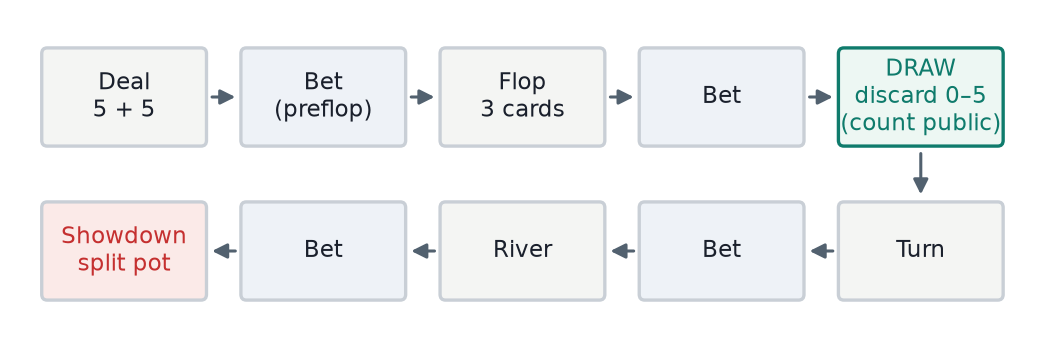
\includegraphics[width=6.45in]{figures/streets.png}
\caption{The street structure of the target game: four betting rounds, one draw round, split-pot showdown.}
\label{fig:streets}
\end{figure}
\end{fullbleed}

\subsection*{Why this game is hard: three separate blow-ups}

\mkey{three blow-ups}Comparing against the games the literature has already conquered isolates exactly what is new. Drawmaha combines three complications that existing work has faced only one at a time:

\begin{center}
\footnotesize
\begin{tabular}{@{}llll@{}}
\toprule
 & Hold'em & Pot-limit Omaha & \textbf{Drawmaha} \\
\midrule
Starting hands & 1{,}326 & 270{,}725 & \textbf{2{,}598{,}960} \\
\quad after suit isomorphism & 169 & $\sim$16{,}500 & \textbf{134{,}459} \\
Draw rounds & 0 & 0 & \textbf{1} (32 discard subsets) \\
Pot & single & single & \textbf{split} (inner + outer) \\
Betting rounds & 4 & 4 & 4 \\
\bottomrule
\end{tabular}
\end{center}

\textbf{Blow-up 1: the hand space.} $\binom{52}{5} = 2{,}598{,}960$ private hands per player --- roughly $2{,}000\times$ hold'em. Dealing both players runs to $\binom{52}{5}\binom{47}{5} \approx 4.0\times10^{12}$ deals before the board or draws multiply it. Every table, buffer, range vector, and dashboard grid in this survey has to survive this number; it is why the project's endgame is a network rather than a table (Section~\ref{sec:deepcfr}), and why a raw DeepStack-style range input does not port (Section~\ref{sec:search}). The one free win is \keyterm{suit isomorphism}\mdef{suit isomorphism}{hands identical up to relabeling suits play identically; merging them is provably lossless}: relabeling suits collapses the 2.6M hands to \textbf{134{,}459} canonical classes --- a $19.3\times$ reduction that costs nothing (Section~\ref{sec:abstraction}).

\textbf{Blow-up 2: the draw round.} The draw inserts a player-\emph{chosen} chance event mid-hand: choosing which of $2^5=32$ subsets to keep is an action; the replacement cards are chance. Its strategic signature is that \hlight{the draw count is public information --- standing pat announces strength (or a bluff, the classic ``snow''), and drawing three announces weakness --- so both players' full draw-count histories belong in the infoset.} The closest solved precedents (2-7 triple draw, badugi) are commercial, not academic; their one loud lesson is that discard \emph{identity} (which cards you threw) drives blocker effects worth real EV (Section~\ref{sec:precedents}).

\textbf{Blow-up 3: the split pot.} Cheapest of the three, and the literature says exactly why: a split pot changes only the \emph{terminal payoff function} --- who gets how much at showdown --- and never the information structure of the tree. Any CFR variant runs unmodified once the leaves pay out correctly; the engineering moves into a fast dual evaluator (inner-hand rank and outer-hand rank per showdown) and into strategy itself becoming two-dimensional: a hand now has inner equity, outer equity, and a scoop probability, which haunts abstraction (Section~\ref{sec:abstraction}) and evaluation units (Section~\ref{sec:evaluation}).

\mnote{Searched: Semantic Scholar, arXiv, GitHub, commercial solver market, poker forums. Nothing for ``Drawmaha'' or ``Sviten Special.''}One more fact frames the whole project: the literature sweep behind this survey searched academic and commercial channels for any Drawmaha solver, bot, or analysis and found \textbf{nothing} --- the game is documented (rules sites, online mixed games) but unstudied. The ``first Drawmaha solver'' claim stands as of August 2026, with a consequence for evaluation: there is no external baseline to beat, so the project must manufacture its own opponents (Section~\ref{sec:evaluation}).

\section{Regret matching: the ten-line rule the whole field runs on}\label{sec:rm}

\mkey{regret matching}Strip poker away entirely and start with rock--paper--scissors. The engine underneath every solver in this survey is a 2000 learning rule by Hart and Mas-Colell called \keyterm{regret matching}\mdef{regret matching}{play each action with probability proportional to its accumulated positive regret}~\cite{hart2000}. After each round, ask for every action: \emph{how much better would I have done had I always played that instead?} Add that gap --- the \keyterm{regret}\mdef{regret}{hindsight gap: (what action $a$ would have paid) $-$ (what I actually got)} --- to a running ledger per action. Next round, play actions in proportion to their positive ledger entries.

\begin{lstlisting}
ledger = {a: 0 for a in ACTIONS}            # cumulative regret per action

def strategy():                              # regret matching
    pos = {a: max(r, 0) for a, r in ledger.items()}
    Z = sum(pos.values())
    return {a: p/Z for a, p in pos.items()} if Z > 0 else uniform()

def update(my_action, their_action):
    for a in ACTIONS:                        # the what-if ledger update
        ledger[a] += payoff(a, their_action) - payoff(my_action, their_action)
\end{lstlisting}

\mnote{\textbf{Rail trace} --- round 1, I throw Rock, they throw Paper (payoff $-1$):\\
what-ifs: Paper $\to 0$, Scissors $\to +1$.\\
ledger: P ${+}{=}\,1$, S ${+}{=}\,2$, R ${+}{=}\,0$\\
next play: P $\tfrac13$, S $\tfrac23$, R $0$.\\
Round 2, I throw Scissors, they hold Paper ($+1$): ledger $\to$ R $-2$, P $0$, S $+2$ --- all-in on Scissors, and the chase begins.}Notice what is \emph{absent}: no learning rate, no optimizer, no gradient --- accumulate and normalize. Hart and Mas-Colell proved this rule is a \keyterm{no-regret learner}\mdef{no-regret learner}{average regret per round provably shrinks toward zero as play continues}: its average regret vanishes over time no matter what the opponent does. That property, not any poker insight, is the load-bearing theorem of computer poker.

Because when \emph{both} players run regret-matching against each other, two things happen at once, and Figure~\ref{fig:rps} shows them with a real simulation. The \emph{current} strategies chase each other forever --- I over-throw Scissors, you learn Rock, I learn Paper, and the ledgers keep circling. But a folk theorem of game theory converts vanishing regret into equilibrium: \hlight{in a two-player zero-sum game, if both players' average regret is $\varepsilon$, the pair of \emph{time-averaged} strategies is a $2\varepsilon$-Nash equilibrium.} The orbit never stops; the \emph{center of the orbit} is the answer. In the figure the running average settles onto exactly $\tfrac13,\tfrac13,\tfrac13$ --- the unexploitable RPS strategy --- while the current strategy never settles at all.

\begin{figure}[t]
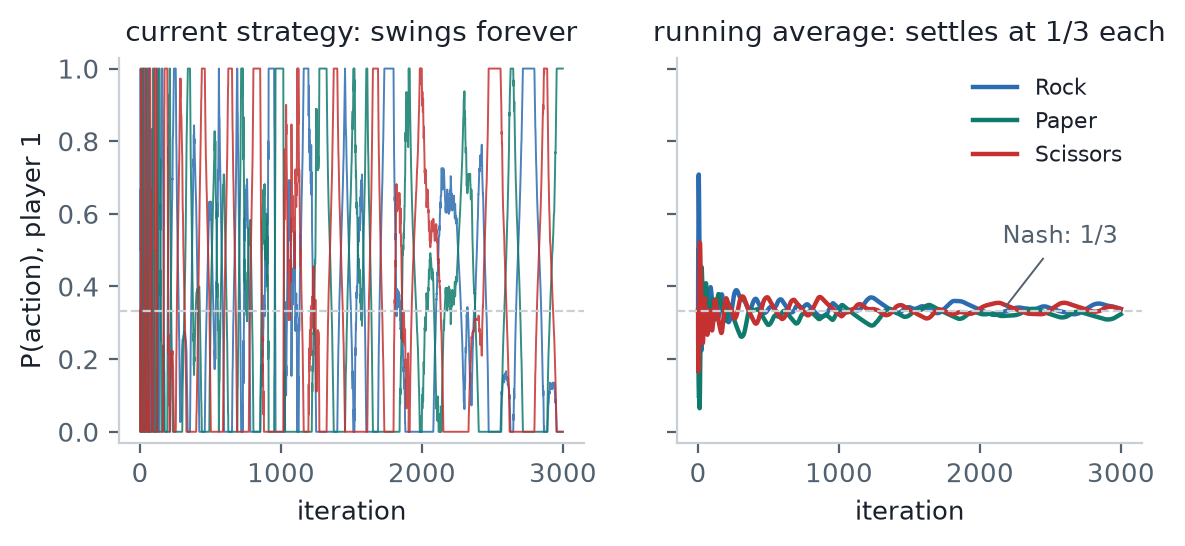
\includegraphics[width=\linewidth]{figures/rps.png}
\caption{Both players running regret matching in rock--paper--scissors (simulated for this paper): current strategy vs.\ its running average.}
\label{fig:rps}
\end{figure}

\pitfall{The single most common conceptual bug in this field is deploying or measuring the current strategy when every guarantee is about the average.} It will reappear in CFR (query the average policy), in Deep CFR (the entire reason an average-policy network exists), and in the RL section (methods that fix cycling by construction so the last iterate \emph{does} converge). Keep the distinction sharp now and the rest of the survey reads easily.

\section{CFR: a little regret-matcher at every decision point}\label{sec:cfr}

\mkey{counterfactual regret}Regret matching handles one simultaneous decision. Poker is a \emph{tree} of sequential decisions under hidden information, and the naive fix --- treat every complete game plan as one giant ``action'' and regret-match over plans --- explodes combinatorially. The 2007 breakthrough of Zinkevich, Johanson, Bowling, and Piccione~\cite{zinkevich2007} is \keyterm{counterfactual regret minimization}\mdef{CFR}{run an independent regret-matcher at every infoset; their local regrets provably bound global regret}: put an \emph{independent} little regret ledger at every information set, define each one's regret the right way, and prove the sum of the local regrets upper-bounds the global regret of the whole strategy. Minimize locally, win globally --- then the folk theorem from Section~\ref{sec:rm} converts the vanishing regret into a converging \emph{average} strategy.

The one subtlety is what ``the right way'' means, and it is where the name comes from.

\begin{intuition}{counterfactual value: score the spot as if you had steered to it}
An infoset deep in the tree is only reached some of the time, and partly because of \emph{your own} earlier choices. If local regrets were weighted by how often \emph{you} actually go there, a spot you currently avoid would accumulate no regret and never be reconsidered --- learning would freeze. So CFR scores each infoset \emph{counterfactually}: weight its value by the probability that \emph{the opponent and the deck} let you arrive (their reach), while pretending you steered there with probability one. Your own choices never gate their own reconsideration; the opponent's play and the cards set the stakes. That reach-weighting detail is the entire trick --- and getting it backwards is the classic silent implementation bug (Section~\ref{sec:engineering}).
\end{intuition}

In symbols, for infoset $I$ with strategy $\sigma_t$ at iteration $t$, action $a$'s instantaneous regret is
$$ r_t(I,a) \;=\; \pi^{\sigma_t}_{-i}(I)\,\bigl[\,v(I,a) - \textstyle\sum_{a'} \sigma_t(I,a')\,v(I,a')\,\bigr], $$
where $\pi^{\sigma_t}_{-i}(I)$ is the opponent-and-chance reach probability and $v(I,a)$ the expected payoff after taking $a$ at $I$. Each ledger accumulates $R_T(I,a)=\sum_t r_t(I,a)$; regret matching over $R_T^+$ gives the next strategy; and the guarantee is exploitability of the \emph{average} strategy shrinking as $O(1/\sqrt{T})$.

\begin{lstlisting}
def cfr(state, reach_me, reach_opp):         # one traversal, my update
    if state.terminal(): return state.payoff()
    I = infoset(state)                        # my cards + public history
    sigma = regret_match(ledger[I])
    v = {a: cfr(state.play(a), ...) for a in I.actions}   # recurse
    ev = sum(sigma[a] * v[a] for a in I.actions)
    if I.player == me:
        for a in I.actions:                   # counterfactual weighting
            ledger[I][a]     += reach_opp * (v[a] - ev)
        avg_ledger[I][sigma] += reach_me      # average strategy, own reach
    return ev
\end{lstlisting}

\mkey{kuhn poker}The standard first proving ground is \keyterm{Kuhn poker}\mdef{Kuhn poker}{3-card deck (J,Q,K), one card each, one bet of 1; the smallest real poker game}: twelve infosets, yet genuine hidden information, value betting, and an equilibrium that \emph{must} bluff (the jack bluffs one-third as often as the king value-bets). Its equilibrium is known in closed form, so an implementation can be checked to the digit. Figure~\ref{fig:kuhn} shows CFR solving it live for this paper, and the plot restates every claim of the last two sections with real data: the average strategy's exploitability marches down the $1/\sqrt{T}$ guide toward zero; the \emph{current} strategy of vanilla CFR stays stuck around $0.2$ chips/hand forever, cycling exactly as the theory predicts.\mnote{The simulation behind Fig.~\ref{fig:kuhn} reproduces Kuhn's game value $-1/18\approx-0.0556$ for the first player to 4 decimal places --- the kind of closed-form check Section~\ref{sec:engineering} argues every implementation needs.}

\begin{figure}[t]
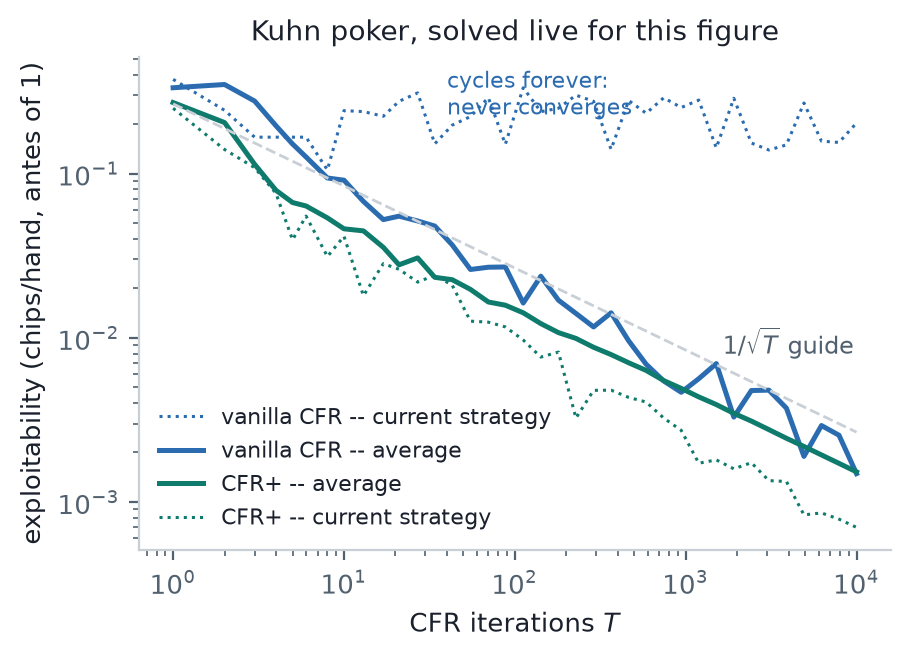
\includegraphics[width=\linewidth]{figures/kuhn_cfr.png}
\caption{Real CFR runs on Kuhn poker (computed for this paper): average-strategy exploitability converges; current strategy either cycles (vanilla) or, under CFR+, converges on its own.}
\label{fig:kuhn}
\end{figure}

The figure also previews the next section: the teal curves are \keyterm{CFR+}, a three-tweak variant whose \emph{current} strategy ends up less exploitable than either average --- the empirical surprise that made million-fold-larger games solvable.

Two closing notes calibrate expectations. First, cost: vanilla CFR walks the \emph{entire} tree every iteration --- fine for Kuhn's 58 nodes, unthinkable for Drawmaha's $10^{12}$ deals; Sections~\ref{sec:speedups}--\ref{sec:mccfr} are the escape routes. Second, memory: CFR stores two numbers per infoset-action (regret sum, strategy sum). That linear-in-infosets footprint is precisely what made $10^{12}$-state abstractions of limit hold'em solvable in 2007 where LP solvers managed $10^{8}$ --- and precisely what runs out at Drawmaha scale, forcing Section~\ref{sec:deepcfr}.

\section{The tabular speedups: CFR+, discounting, pruning, vectorization}\label{sec:speedups}

\mkey{cfr+}Everything after 2007 is an efficiency layer on the same skeleton, and the layers compound. They matter to this project twice: the toy-game and mini-drawmaha phases will literally run them, and Deep CFR silently inherits their weighting ideas.

\textbf{CFR+ (Tammelin 2014)}~\cite{tammelin2014,tammelin2015} is three small changes applied \emph{together}: (1) \emph{regret-matching+}: clip each ledger entry at zero after every iteration, so an action buried under old negative regret can come back the moment it turns good, instead of slowly paying down debt; (2) \emph{alternating updates}: update one player per traversal, so each responds to the other's freshest strategy; (3) \emph{linear averaging}: weight iteration $t$'s contribution to the average by $t$, washing out the garbage early iterations. The provable rate is unchanged ($O(1/\sqrt{T})$), but empirical convergence often looks like $1/T$ or better --- visible in Figure~\ref{fig:kuhn}, where CFR+'s \emph{current} strategy beats every average curve. CFR+ is what solved full heads-up limit hold'em: \textbf{Cepheus} (2015)~\cite{bowling2015} drove a $10^{14}$-infoset game below 1 milli-big-blind/hand of exploitability using 4{,}800 CPUs for 68 days --- both the triumph of the tabular approach and the clearest statement of its ceiling. \pitfall{Cherry-picking one of the three tweaks (say, clipping alone with uniform averaging) can converge slower than vanilla CFR --- they are specified as a package.}

\textbf{Discounted CFR (Brown \& Sandholm 2019)}~\cite{brown2019dcfr} generalizes the idea: scale positive regrets by $t^\alpha/(t^\alpha{+}1)$, negative by $t^\beta/(t^\beta{+}1)$, average-strategy contributions by $(t/(t{+}1))^\gamma$. The recommended $(\alpha,\beta,\gamma)=(1.5,\,0,\,2)$ beat CFR+ in every game tested --- the first algorithm to do so. Its sibling \textbf{Linear CFR} (everything weighted by $t$) matters for a different reason: it is the member that stays sound under \emph{sampling}, and Deep CFR builds on exactly that weighting. The rule of thumb the literature converged on: \hlight{full traversals $\to$ DCFR$(1.5,0,2)$; anything sampled $\to$ linear weighting.}

Three more tools complete the tabular kit:

\begin{itemize}
\item \textbf{Regret-based pruning} (Brown \& Sandholm)~\cite{brown2015pruning}: temporarily skip traversing subtrees hanging off actions with deeply negative regret --- they contribute nothing to the current strategy --- and revisit them occasionally in case they recover. Large constant-factor savings; used inside the Libratus/Pluribus blueprints.
\item \textbf{Vector-form / public chance sampling} (Johanson et al.\ 2012)~\cite{johanson2012pcs}: traverse the \emph{public} tree once while carrying a vector of values for \emph{every} private hand simultaneously --- turning thousands of scalar traversals into one matrix-shaped pass. This is the trick behind PioSolver-class speed and behind fast exact best-response computation (Section~\ref{sec:evaluation}). For Drawmaha the private-hand vector is 134{,}459 entries (canonical classes) instead of hold'em's 1{,}326 --- painful but not absurd on a GPU.
\item \textbf{Sequence-form LP} (Koller, Megiddo \& von Stengel 1994--96)~\cite{koller1996}: small games can skip iteration entirely --- an exact linear program solves them to machine precision (the pre-CFR state of the art, alive in the Gambit software). Its modern role is generating \emph{ground truth}: the Leduc value used as a regression constant in Section~\ref{sec:engineering} comes from exactly this.
\end{itemize}

\begin{center}
\footnotesize
\begin{tabular}{@{}lll@{}}
\toprule
Variant & The trick & Use it when \\
\midrule
Vanilla CFR & the 2007 skeleton & learning; debugging \\
CFR+ & clip + alternate + linear avg & full traversals, toy games \\
DCFR$(1.5,0,2)$ & tuned discounting & full traversals, best-in-class \\
Linear CFR & weight everything by $t$ & anything sampled (incl.\ Deep CFR) \\
Pruning & skip hopeless subtrees & big trees, blueprint solves \\
Vector-form & all hands in one public pass & exact solves, best response \\
Sequence-form LP & exact, no iteration & tiny games; ground truth \\
\bottomrule
\end{tabular}
\end{center}

\mnote{Project translation: Kuhn/Leduc run vanilla (to learn) then CFR+/DCFR (to go fast); mini-drawmaha runs sampled linear-weighted MCCFR; Deep CFR inherits the linear weights.}None of this changes the memory wall: every variant above still stores ledgers for every infoset. Two independent escapes exist --- sample the tree so cheap iterations replace exhaustive ones (next section), and shrink or generalize the infoset space itself (Sections~\ref{sec:abstraction}--\ref{sec:deepcfr}).

\section{MCCFR: learn from dealt hands instead of enumerating the universe}\label{sec:mccfr}

\mkey{monte carlo cfr}Vanilla CFR's iteration cost is the whole tree, and Drawmaha's tree is dominated by chance: $\approx 4.0\times10^{12}$ ways to deal the two starting hands, before boards and replacement cards. \keyterm{Monte Carlo CFR}\mdef{MCCFR}{sample part of the tree each iteration; update visited infosets with estimates that are correct on average} (Lanctot et al.\ 2009)~\cite{lanctot2009} replaces ``enumerate every deal'' with ``play sessions'': each iteration samples a slice of the tree and updates only the infosets it visits, using estimates constructed to equal the full-CFR update \emph{in expectation}. Convergence survives (with high probability); iterations get cheaper by orders of magnitude; you take many more of them and win on wall-clock.

The design space is \emph{what to sample}, and Figure~\ref{fig:sampling} draws the two poles:

\begin{figure}[t]
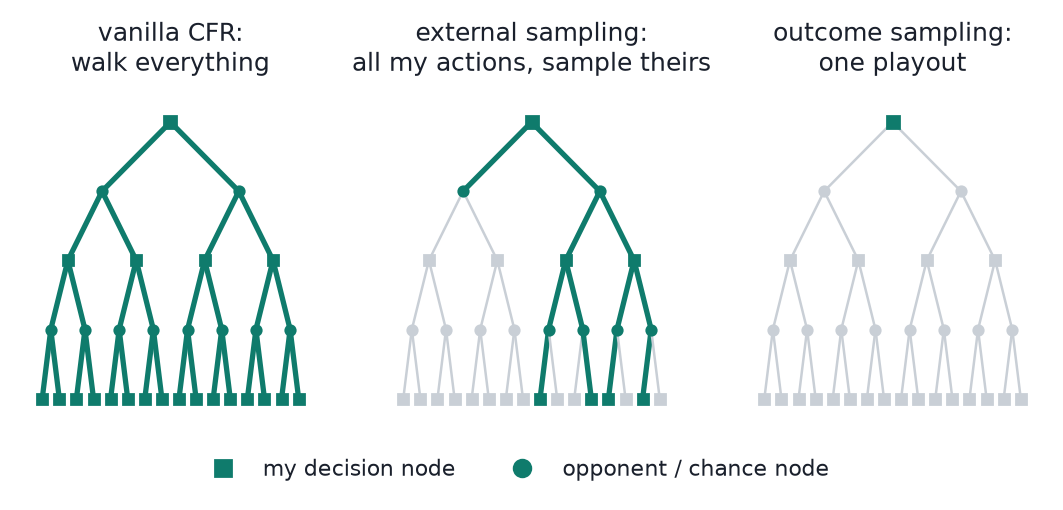
\includegraphics[width=\linewidth]{figures/sampling.png}
\caption{What one iteration touches under each traversal scheme (teal = visited).}
\label{fig:sampling}
\end{figure}

\begin{itemize}
\item \keyterm{External sampling}\mdef{external sampling}{sample chance + opponent choices; traverse ALL of the updating player's own actions}: deal one random hand, sample the opponent's actions from their current strategy, but at \emph{your own} decision points try every action. One iteration costs about one deal plus playouts --- and because everything ``external'' to you was sampled at its true probability, the estimates need \textbf{no importance-weight corrections at all}. Low variance, simple, the practitioner default.
\item \keyterm{Outcome sampling}\mdef{outcome sampling}{sample a single playout, everything included; correct with importance weights}: sample one complete playout including your own actions. Cheapest possible iteration --- and the estimate must be divided by the probability of having sampled that path, an \keyterm{importance weight}\mdef{importance weight}{1/(probability of the sampled path): rescales a sampled outcome so its average is unbiased} that explodes as strategies sharpen and probabilities shrink. High variance is the price of touching one path.
\end{itemize}

\begin{intuition}{importance weights are an honest bookkeeper with a loud voice}
If you only visit a spot 1\% of the time, the rare visit must count $100\times$ to keep the average honest --- that division by the sampling probability is all an importance weight is. The bookkeeping is exactly right \emph{on average} and horribly noisy per sample: one rare visit slams the ledger. External sampling's quiet superpower is never needing the correction for your own actions (you tried them all), which is why the variance stays tame --- and why Deep CFR chooses it (Section~\ref{sec:deepcfr}).
\end{intuition}

\begin{lstlisting}
def traverse(state, me):                     # external-sampling MCCFR
    if state.terminal(): return state.payoff(me)
    I = infoset(state); sigma = regret_match(ledger[I])
    if I.player == me:                       # my node: try EVERY action
        v = {a: traverse(state.play(a), me) for a in I.actions}
        ev = sum(sigma[a] * v[a] for a in I.actions)
        for a in I.actions:
            ledger[I][a] += v[a] - ev        # no importance weights needed
        return ev
    else:                                    # opponent/chance: SAMPLE one
        a = sample(sigma if I.player else state.chance_dist())
        avg_ledger[I][sigma] += 1            # opponent's avg-strategy bookkeeping
        return traverse(state.play(a), me)
\end{lstlisting}

For an RL-trained reader, one bridge makes the whole variance topic familiar: \textbf{VR-MCCFR} (Schmid et al.\ 2019)~\cite{schmid2019vr} subtracts a learned per-infoset \emph{baseline} from sampled values and adds it back in expectation --- literally the control-variate/advantage-baseline trick from policy-gradient RL, imported wholesale. Reported effect: variance down $\sim1000\times$, an order-of-magnitude speedup, and the first working marriage of sampling with CFR+-style updates. It is an optimization, not a correctness requirement --- the note for the project is simply that \mnote{if mini-drawmaha MCCFR converges too slowly, noise is the first suspect and baselines are the literature's fix.}plain external sampling already converges.

Two practical rules close the section. \hlight{If you own the simulator --- and this project does --- external sampling is the default; outcome sampling exists for black-box environments and pays a variance tax that takes a whole extra learned network to tame} (DREAM, Section~\ref{sec:deepcfr}). And under sampling, use \emph{linear} weighting rather than CFR+'s clipping (Section~\ref{sec:speedups}): clipping interacts badly with noise, a lesson that carries straight into Deep CFR's buffers. Middle grounds exist (``robust sampling'' traverses $k$ of your actions instead of all --- a compute/variance dial worth remembering if Drawmaha's 32-subset draw node makes full external traversal expensive), but external sampling is where this project starts.

\section{Abstraction: deciding which hands share a strategy}\label{sec:abstraction}

\mkey{abstraction}Sampling makes iterations affordable; the ledgers themselves still need one row per infoset. The classical answer is \keyterm{abstraction}\mdef{abstraction}{solve a smaller merged game whose solution transfers back to the real one}: merge strategically similar situations, solve the smaller game, lift the strategy back. A decade of poker research is essentially a ratchet of better answers to ``which hands should share a row?'' --- and even though this project's endgame replaces tables with networks, the ratchet survives as the checklist for what the network's \emph{inputs} must express, and as the recipe for the dashboard's bucketed range view.

\textbf{Layer 0 --- lossless.} Some merges cost literally nothing: hands identical up to relabeling suits play identically, and Gilpin \& Sandholm~\cite{gilpin2007} proved equilibria of the merged game lift back \emph{exactly}. For Drawmaha the sweep behind this survey brute-force-verified the payoff: the 2{,}598{,}960 five-card hands collapse to exactly \textbf{134{,}459} canonical classes ($19.3\times$). \hlight{Suit-isomorphic canonicalization is free accuracy --- it should key every table, buffer, and dashboard lookup in the project regardless of any other choice.} One caveat travels with it: the $19.3\times$ shrinks as board and draw cards pin suits down --- late-street symmetry is weaker, and Waugh's perfect-indexing algorithm~\cite{waugh2013iso} is the standard way to key the canonical classes.

\textbf{Layer 1 --- a scalar per hand.} Rank every hand by \keyterm{E[HS]}\mdef{E[HS]}{expected hand strength: equity vs.\ a random opponent hand, averaged over runouts} and cut into percentile buckets. Trivial to compute, fine for a first prototype --- and blind in a specific, poker-relevant way: a made hand and a big draw can carry the \emph{same} average equity with \emph{opposite} distributions (Figure~\ref{fig:equity}), and they want opposite strategies (one wants the pot now; the other prices in cards to come).

\begin{figure}[t]
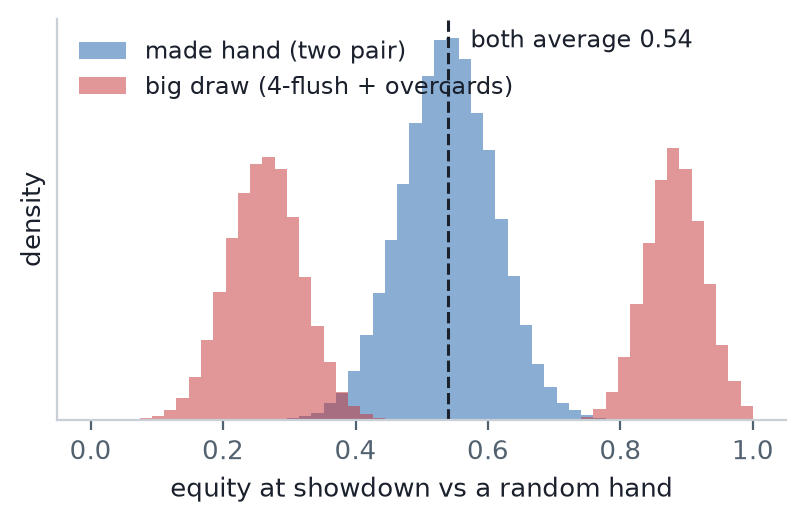
\includegraphics[width=\linewidth]{figures/equity.png}
\caption{Two hands with equal average equity and opposite equity distributions (illustrative densities): the scalar cannot see the difference; the histogram can.}
\label{fig:equity}
\end{figure}

\textbf{Layer 2 --- the distribution.} Represent each hand by its full equity \emph{histogram} over runouts and cluster the histograms with $k$-means under \keyterm{earth mover's distance}\mdef{earth mover's distance}{distance between histograms = minimum ``work'' to shovel one shape into the other} (Johanson et al.\ 2013~\cite{johanson2013}). Distribution-aware buckets beat scalar buckets on both exploitability and head-to-head play. The same study validated \keyterm{imperfect recall}\mdef{imperfect recall}{let the abstraction forget earlier-street details to spend its bucket budget on the present} --- strictly better use of a fixed budget, at the cost of voiding CFR's convergence guarantee (it works empirically; Section~\ref{sec:solving}'s perfect-recall condition is the reason the theory breaks).

\textbf{Layer 3 --- the trajectory.} Two hands can even share a final histogram but \emph{realize} it differently --- exactly the pre-draw/post-draw distinction. Potential-aware abstraction (Ganzfried \& Sandholm 2014~\cite{ganzfried2014}, the champion-agent method) represents an early-street hand by its distribution over \emph{next-street buckets}, built bottom-up, so when strength arrives matters, not just how much. \mnote{Drawmaha translation: pre-draw buckets should be distributions over post-draw buckets --- one recursive level, since there is one draw. This is literally the situation the method was invented for.}

\textbf{Actions get abstracted too.} A pot-limit tree still needs a bet-size menu (the project's v1: \{pot\} only, by design), and any \emph{deployed} strategy must interpret off-menu sizes. The standard is the \keyterm{pseudo-harmonic mapping}\mdef{action translation}{rule mapping a real-world bet onto the solver's nearest menu sizes} (Ganzfried \& Sandholm 2013~\cite{ganzfried2013at}): randomize between the neighboring menu sizes with game-theoretically derived probabilities --- naive nearest-size rounding is provably exploitable by bet sizing alone. The dashboard needs this the day it accepts a user-typed bet; the principled upgrade is re-solving off-menu spots exactly (Section~\ref{sec:search}).

Two warnings temper the whole enterprise. First, the \textbf{abstraction pathology} (Waugh et al.\ 2009~\cite{waugh2009}): \pitfall{refining an abstraction --- more buckets, finer distinctions --- can make the real-game strategy MORE exploitable; quality is non-monotonic in size}, so bucket sweeps must be validated by measured exploitability, never assumed. Second, the modern question --- \emph{doesn't deep learning make all this obsolete?} --- gets a precise answer: Deep CFR's paper claims it ``obviates the need for abstraction,'' and what it actually removes is the hand-crafted \emph{clustering}. The \emph{representation} problem survives inside the input featurization: canonical hands, card embeddings, street and pot features are abstraction moved into the network's first layer, and everything this section learned --- distribution shape matters, trajectory matters, and for Drawmaha strength is \textbf{two-dimensional} (inner equity, outer equity, scoop probability, so a scalar is even more misleading than in hold'em) --- is the checklist for those features.

\mnote{The display side reuses this machinery: an equity-histogram $k$-means into 8--20 \emph{named} buckets over the 134,459 classes is the planned range-view grouping, even though the solver itself is bucket-free.}For this project abstraction therefore lives in three places: free canonicalization everywhere; honest bucketing (layers 1--3) for the tabular mini-drawmaha stage; and feature design plus the dashboard's human-readable buckets at full scale.

\section{Deep CFR: the ledger becomes a regression problem}\label{sec:deepcfr}

\mkey{deep cfr}Now the pieces assemble into the project's centerpiece. At full Drawmaha scale no table fits, and \keyterm{Deep CFR}\mdef{Deep CFR}{CFR where neural networks predict the regret ledger's contents instead of storing them} (Brown, Lerer, Gross \& Sandholm 2019~\cite{brown2019deep}) makes the one substitution left to make: everything about CFR stays --- external-sampling traversals, regret matching, average-vs-current --- but the per-infoset ledger is replaced by a network trained to \emph{predict} what the ledger would contain, generalizing across the millions of hands that were never sampled. The bet is statistical: similar hands should regret alike, so every sample teaches a neighborhood, and bucketing is learned end-to-end instead of hand-engineered. It was the first non-tabular CFR to work in large poker, beating NFSP on exploitability (37 vs.\ 47 mbb/hand on Flop Hold'em) and playing competitively against a $3.3\times10^8$-bucket abstraction in full limit hold'em.

\begin{figure}[t]
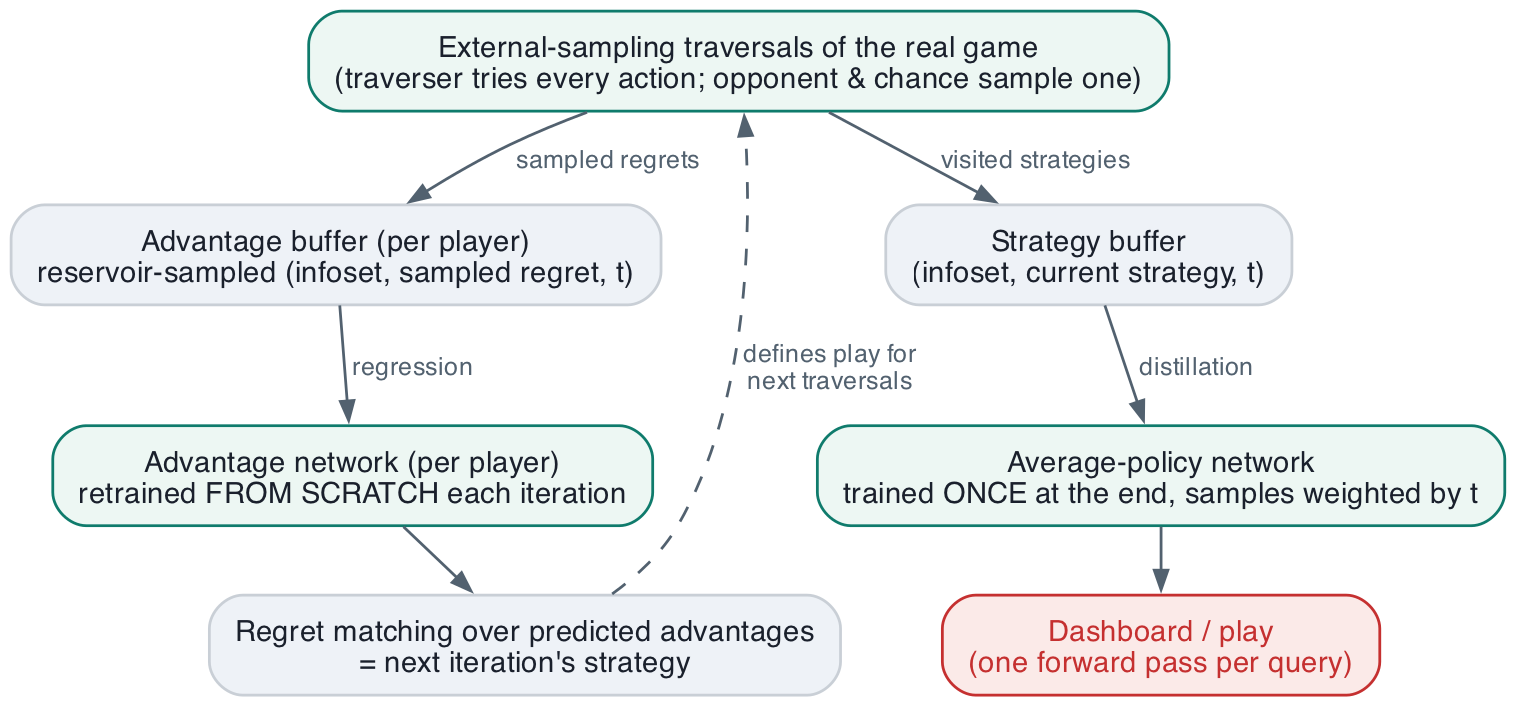
\includegraphics[width=\linewidth]{figures/pipeline.png}
\caption{The Deep CFR training loop; teal = learned components, red = what the dashboard queries.}
\label{fig:pipeline}
\end{figure}

Walking Figure~\ref{fig:pipeline} clockwise:
\begin{enumerate}
\item \textbf{Traverse.} Run external-sampling traversals of the \emph{real} game (Section~\ref{sec:mccfr}); the current strategy at any infoset is regret matching over the advantage network's predictions.
\item \textbf{Collect.} Each traversal writes (infoset features, sampled instantaneous regret, iteration $t$) tuples --- \keyterm{advantages}\mdef{advantage (CFR sense)}{a sampled instantaneous counterfactual regret; the regression target, NOT actor--critic's advantage} --- into a per-player buffer, and (infoset, current strategy, $t$) into a strategy buffer.
\item \textbf{Regress.} Each iteration trains that player's advantage network \emph{from scratch} on its buffer. From scratch is not paranoia: cumulative regrets are nonstationary, and the paper's ablation shows fine-tuning one network across iterations converges substantially worse.
\item \textbf{Average.} At the very end, one \keyterm{average-policy network}\mdef{average-policy network}{a net distilled from all iterations' strategies, weighted by $t$ --- the deployable equilibrium approximation} is distilled from the strategy buffer with samples weighted by $t$ (Linear-CFR weighting, Section~\ref{sec:speedups}). \hlight{That single network IS the solver output --- the thing the folk theorem blesses, the thing the dashboard queries at one forward pass per hand.}
\end{enumerate}

\begin{intuition}{reservoir buffers: a fair fixed-size memory of an endless stream}
The buffers cannot hold every sample ever generated, and a FIFO buffer would remember only recent iterations --- but the \emph{average} strategy needs all of history represented fairly. Reservoir sampling keeps a fixed-size buffer that is, at every moment, a uniform random sample of everything seen so far: each new item displaces a random resident with exactly the right probability. Deep CFR's guarantees lean on this fairness; swapping in a FIFO buffer is a known way to quietly break convergence.
\end{intuition}

\begin{lstlisting}
for t in 1..T:                                # Deep CFR outer loop
  for p in players:
    for k in 1..K:                            # e.g. K = 10,000 traversals
      traverse(deal(), p, adv_net[p], adv_buf[p], strat_buf, t)
    adv_net[p] = train_from_scratch(adv_buf[p],   # regression on
                   target="sampled regret", weight="t")  # ledger contents
final = train(strat_buf, target="strategy", weight="t")  # average-policy net
# play/dashboard: sigma(I) = regret_match(final(I))  -- one forward pass
\end{lstlisting}

\subsection*{The published recipe, as starting hyperparameters}

Deep CFR's appendix is a de-risked starting point, small enough to be encouraging:

\begin{center}
\footnotesize
\begin{tabular}{@{}ll@{}}
\toprule
Network & 7 layers, $\sim$99K parameters: card branch + bet branch \\
Card encoding & rank + suit + card embeddings, summed within permutation-invariant groups \\
Bet encoding & per betting slot: occurred-flag + bet size as pot fraction \\
Buffers & 40M samples each (advantage $\times2$, strategy), reservoir-sampled \\
Per iteration & 10K traversals; retrain 4K SGD steps, batch 10K \\
Optimizer & Adam, lr $10^{-3}$, gradient-norm clip 1 \\
Small-game anchor & (SD-CFR, Leduc): $3\times64$ nets, 1M buffers, 1.5K traversals/iter \\
\bottomrule
\end{tabular}
\end{center}

The card-embedding scheme transfers to Drawmaha almost verbatim --- permutation invariance over hole cards only grows in value with 5-card hands --- but two encoding questions have \emph{no} published answer and are flagged now as genuine design work: how the 32-subset \textbf{discard action} should be headed (flat 32-way output vs.\ per-card keep/discard logits --- regret matching over a factorized action space is unexplored territory), and how both players' public \textbf{draw-count histories} (plus the face-up draw-1 card) enter the input features. Section~\ref{sec:checklist} carries both.

\subsection*{The forks in the neural-CFR family}

\mkey{sd-cfr / dream / escher}Successors map the design space, and three matter here. \textbf{SD-CFR} (Steinberger 2019~\cite{steinberger2019}) deletes the average-policy network: since the average strategy is just an iteration-weighted mixture of per-iteration strategies, and each is recoverable from that iteration's advantage net, storing every checkpoint ($\sim$400KB each) reconstructs the \emph{exact} average --- one less approximation, measurably better exploitability. Its cost is inference: querying means evaluating many checkpoints, awkward for a live dashboard. \mnote{Best of both, and the plan: train SD-CFR-style (keep checkpoints, evaluate exactly), distill ONE average-policy net at the very end for serving.}\textbf{DREAM} (2020~\cite{steinberger2020dream}) and \textbf{ESCHER} (2022~\cite{mcaleer2022}) exist for simulator-free settings: outcome sampling forces importance weights, whose variance takes an extra learned baseline network (DREAM) or a learned history-value function under a fixed sampling policy (ESCHER) to control. Their lesson for a project that \emph{owns} its simulator is purely diagnostic: \hlight{importance-sampling variance is what kills neural CFR at scale --- choose external sampling on day one and the whole problem never appears.}

Two pitfalls close the section, both documented failure modes. \pitfall{Forgetting the iteration-$t$ weighting on strategy-buffer samples silently converges to the wrong average} --- a classic bug, since nothing crashes. And the loss curves of advantage networks are \emph{expected} to look bad: cumulative regrets grow and drift across iterations (the nonstationarity ReCFR~\cite{liu2022recfr} formalizes), so a plateauing or climbing regression loss is often target drift, not optimizer failure --- one more reason Section~\ref{sec:evaluation} insists exploitability curves, never training losses, are the progress signal.

\section{The other lineage: search at play time, value networks at the horizon}\label{sec:search}

\mkey{why search is hard here}Deep CFR \emph{amortizes}: all solving happens in training, and play is a forward pass. The rival lineage --- the one behind DeepStack, Libratus, and today's GTO Wizard AI --- \emph{searches}: solve the situation you are actually in, at play time, the way chess engines do. In poker that idea breaks twice before it works. First, you never know which state you are in, so search must reason over \emph{ranges} (Section~\ref{sec:solving}'s probability cloud) rather than positions. Second, and less obviously:

\begin{intuition}{why you cannot just solve the river when you get there}
How an opponent plays a river depends on rivers that never happened --- if your new river strategy stops paying off their bluffs, then \emph{arriving} at this river with bluffs was a mistake for them, and a rational opponent's whole earlier game shifts. Solve the subgame ``optimally'' in isolation and you can make your \emph{overall} strategy more exploitable. The 2014 fix (Burch et al.~\cite{burch2014}) is a buyout clause: re-solve the subgame under a constraint that at its entrance, every opponent hand may either play on into your new strategy or take a ``buyout'' equal to what that hand was worth under your old strategy. If no hand prefers deviating, your new strategy concedes nothing it had not already conceded --- \emph{safe re-solving}, the gadget every sound search method builds on.
\end{intuition}

With safety available, the lineage is a sequence of ways to stop searching early (Figure~\ref{fig:lineage} maps it):

\begin{itemize}
\item \textbf{DeepStack} (2017~\cite{deepstack}): re-solve a small lookahead at \emph{every} decision (``continual resolving''), carrying only your range and the opponent's buyout values forward; where the lookahead ends, a \keyterm{counterfactual value network}\mdef{counterfactual value net}{maps (pot, board, both ranges) $\to$ per-hand values --- a learned evaluation function over ranges} estimates the rest. First expert-level HUNL win; the net's input is both players' full range vectors.
\item \textbf{Libratus} (2017~\cite{libratus}): superhuman with \emph{zero} neural networks --- an abstraction blueprint (MCCFR), plus \emph{nested} safe re-solving that spawns a finer subgame solve every time the opponent does anything (including bet sizes outside the blueprint's menu, retiring action translation), plus overnight self-repair of the blueprint where opponents probed. Proof that search, not deep learning, was the load-bearing superhuman ingredient.
\item \textbf{Depth-limited solving} (2018~\cite{brown2018dls}): the cheap trick --- at the depth limit, instead of a value net, let the opponent choose among a handful of precomputed \emph{continuation strategies} (an adversarial ``several ways the rest could play''). Modicum beat top prior bots on a 4-core laptop; Pluribus (2019~\cite{pluribus}) rode the same recipe to 6-max on commodity hardware.
\item \textbf{ReBeL} (2020~\cite{rebel}): the clean theory --- recast poker as a perfect-information game over \keyterm{public belief states}\mdef{public belief state}{public observations + both players' hand distributions: a state everyone CAN see} and run AlphaZero's loop (self-play + search + value/policy nets) on that transformed game, with a Nash convergence proof. \textbf{Student of Games} (2023~\cite{sog}) generalized the recipe to chess, Go, HUNL, and Scotland Yard with one algorithm.
\item \textbf{GTO Wizard AI} (commercial, ex-Ruse~\cite{gtowizardai}): the deployed endpoint --- solves street-by-street in real time with self-play-trained value networks standing in for future streets; self-reported: arbitrary stacks and bet sizes, $\sim$3s per street, rivers solved exactly, +19.4bb/100 over Slumbot. No paper, so treat all numbers as vendor claims; the \emph{architecture pattern} is the public part.
\end{itemize}

\begin{fullbleed}
\begin{figure}[t]
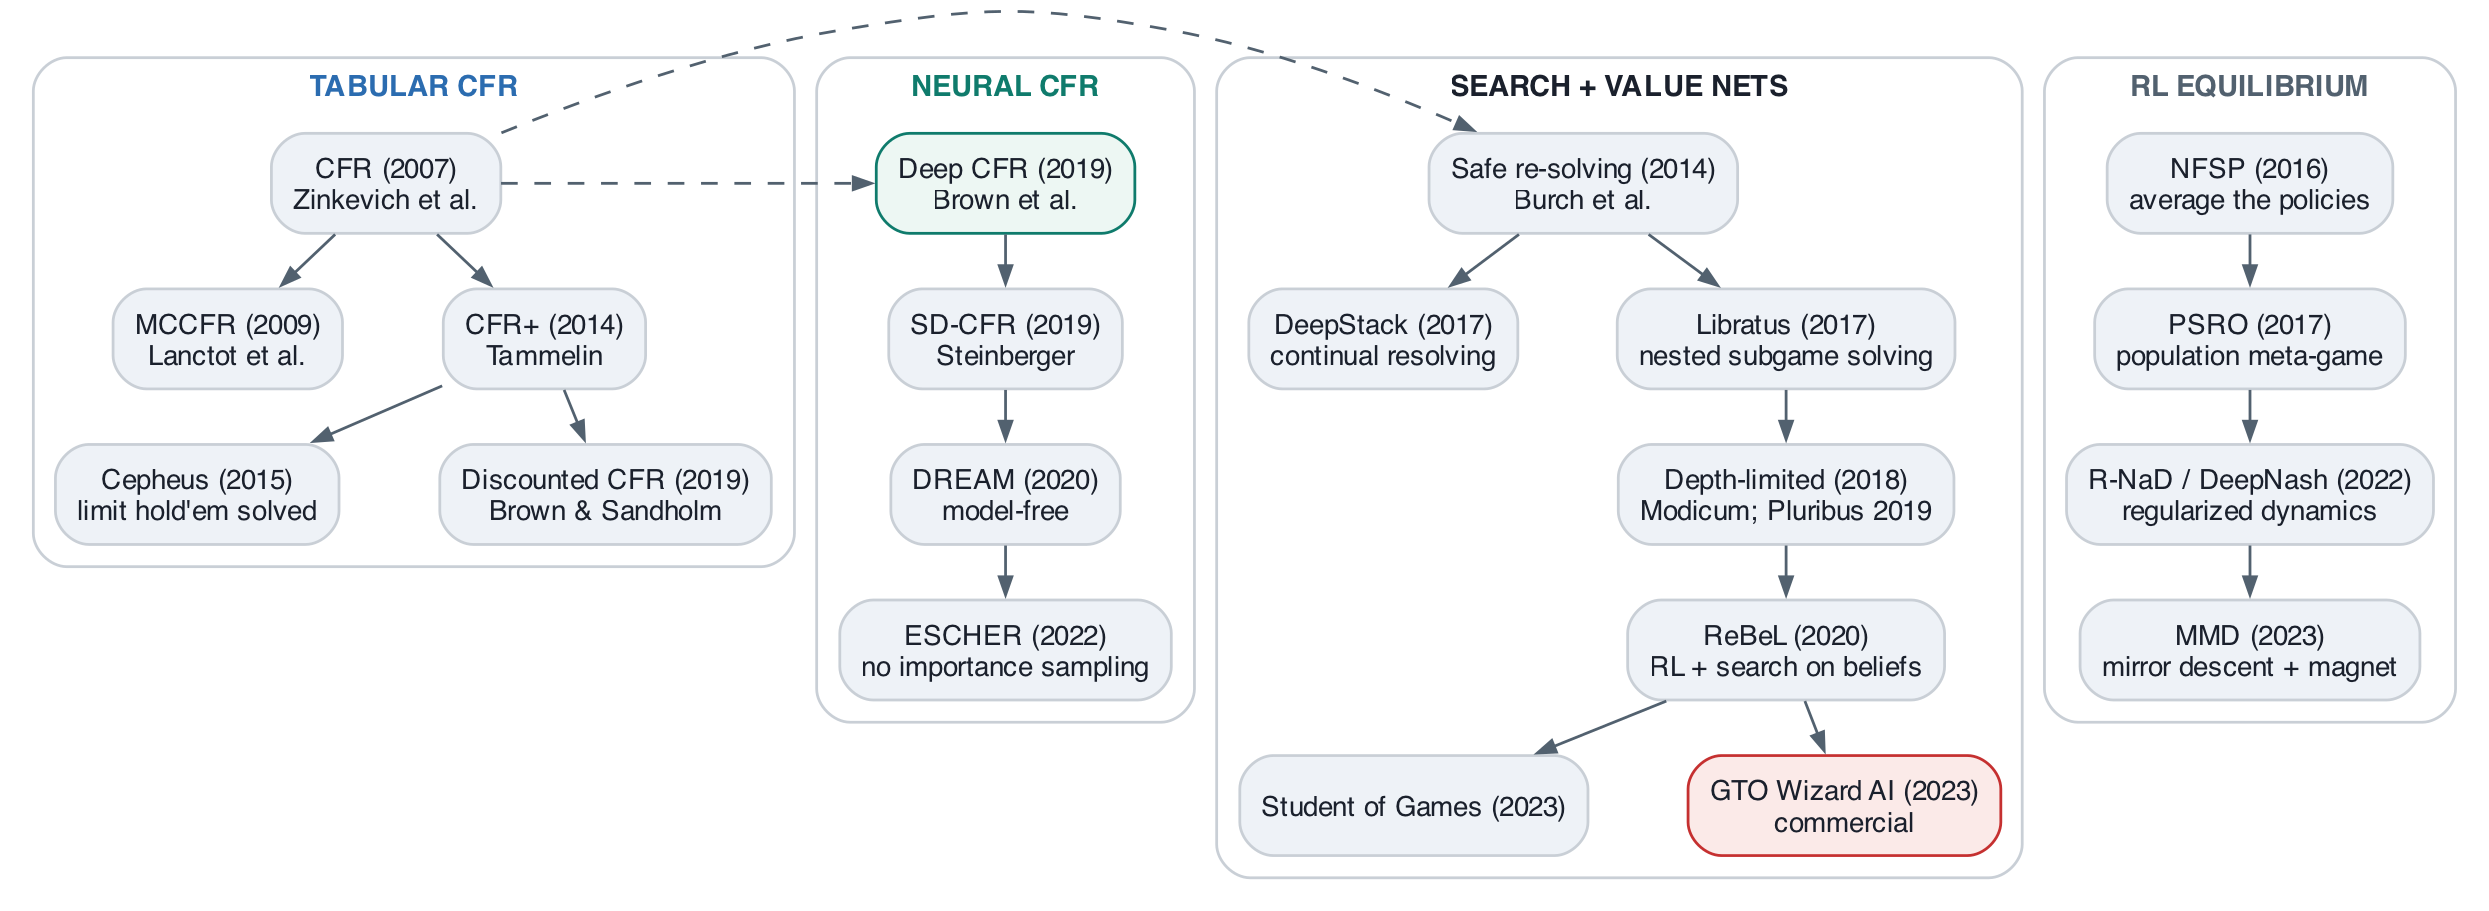
\includegraphics[width=6.45in]{figures/lineage.png}
\caption{The four method families and their landmark systems; dashed arrows mark CFR's ideas feeding the other lineages.}
\label{fig:lineage}
\end{figure}
\end{fullbleed}

\subsection*{Amortized vs.\ search: the actual tradeoff, and the Drawmaha verdict}

\begin{center}
\footnotesize
\begin{tabular}{@{}lll@{}}
\toprule
 & Amortized policy (Deep CFR) & Search + values (DeepStack/ReBeL) \\
\midrule
Per-query cost & one forward pass, ms & a subgame solve, seconds \\
Errors at play & baked in at training & partially corrected by search \\
Off-menu spots & needs action translation & re-solves them natively \\
Engineering & one training loop & belief tracking + gadgets + nested solves \\
Range input & never materialized & \textbf{2{,}598{,}960-dim vectors} \\
\bottomrule
\end{tabular}
\end{center}

\mkey{the 2.6M-dim wall}The last row is the Drawmaha-specific wall: every neural system in this lineage feeds \emph{range vectors} into its networks --- 1{,}326 dimensions in hold'em, \textbf{2{,}598{,}960} in Drawmaha (5.2M for both players). Nothing ports without aggressive hand bucketing or a factorized belief representation first, and that is the single biggest open design problem for any future Drawmaha search layer. Working in search's favor: the public draw count slots perfectly into public-belief-state bookkeeping, pot-limit bounds the bet-size branching, and the post-draw game is comparatively small. \mnote{Ranked future upgrades, cheapest first: (1) depth-limited resolve at the draw boundary using the Deep CFR net $\pm$ perturbations as continuation strategies; (2) a post-draw value net, DeepStack-style; (3) full belief-state search.}\hlight{The project's verdict, echoing the commercial history: amortized Deep CFR first --- search is the accuracy upgrade you buy later, not the foundation you start on.} One honest caveat travels with any future resolve layer: updating the opponent's range \emph{through} a hidden discard (they drew two --- which two?) is a belief-update computation no paper writes down for poker draws; Section~\ref{sec:checklist} carries it as an open problem.

\section{Where actor--critic fits: the RL road to equilibrium, and its potholes}\label{sec:rl}

\mkey{why ppo self-play fails}A reader arriving from applied RL asks the obvious question: why not just PPO in self-play --- policy network, value critic, reward = chips, train against a copy of yourself? The answer is a theorem, not a tuning problem. Perolat et al.~\cite{perolat2020} proved that the idealized dynamics of gradient self-play in two-player zero-sum imperfect-information games are \emph{Poincar\'e-recurrent}: trajectories \textbf{orbit} the equilibrium and return arbitrarily close to where they started, forever. The learning vector field \emph{rotates} around the solution instead of pointing at it (Figure~\ref{fig:cycle}, left) --- rock--paper--scissors chasing, at scale, in your GPU bill. \pitfall{Cycling in zero-sum self-play is geometry, not a hyperparameter problem: no learning-rate schedule fixes a field with no attraction.} The deep reason is Section~\ref{sec:solving}'s fact 2: equilibria are \emph{mixed}, and ``improve greedily against the current opponent'' has no mixed fixed point to settle into.

\begin{figure}[t]
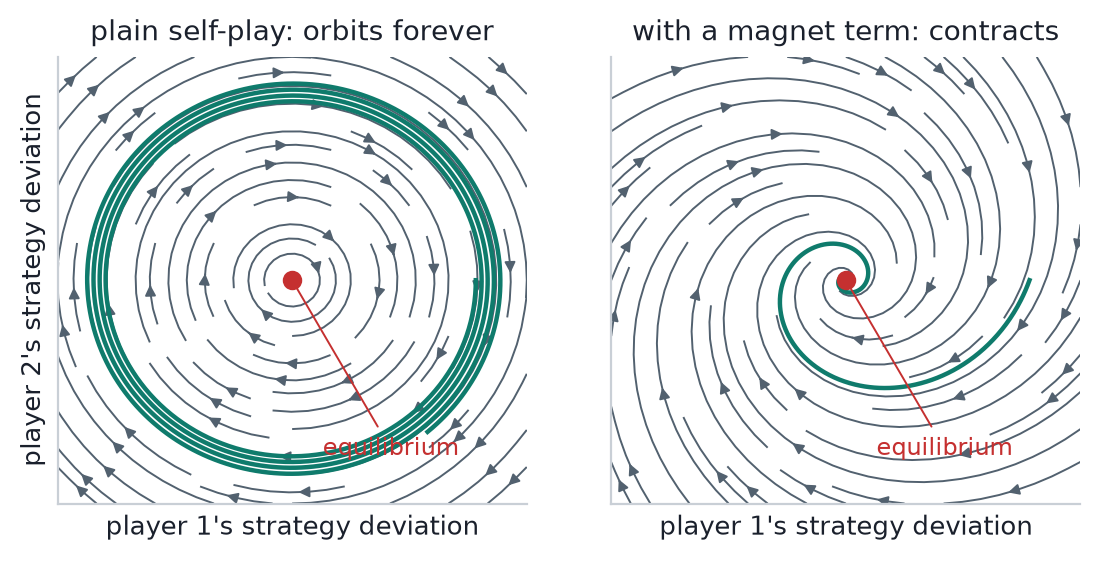
\includegraphics[width=\linewidth]{figures/cycle.png}
\caption{Real trajectories of the two dynamics (simulated for this paper): unregularized self-play orbits; adding a KL pull toward a reference policy makes the same dynamics contract.}
\label{fig:cycle}
\end{figure}

Contrast the games where naive self-play \emph{does} work --- AlphaZero's chess, shogi, Go~\cite{alphazero}. Perfect information supplies two pillars: every state has a minimax value independent of beliefs (so a value target exists), and a deterministic optimal policy exists (so greedy improvement is a genuine ladder). Hidden cards demolish both --- values depend on ranges, ranges on both strategies, and optimal play must randomize. Everything that works in imperfect information restores convergence by one of three escapes:

\begin{center}
\footnotesize
\begin{tabular}{@{}p{0.62in}p{1.02in}p{2.86in}@{}}
\toprule
Escape & Method & Mechanism, and its cost \\
\midrule
\textbf{Average} & NFSP (2016)~\cite{nfsp} & DQN best-responds to the opponent's \emph{historical average} policy; a supervised net learns that average and is what you deploy. Cost: slow; beaten by Deep CFR. \\
\textbf{Population} & PSRO (2017)~\cite{psro} & meta-game over whole trained policies: solve the small matrix, train a new RL best response to the mixture, repeat. Cost: a full RL run per iteration; coarse at poker's fine mixing. \\
\textbf{Regularize} & R-NaD / DeepNash (2022)~\cite{deepnash}; MMD (2023)~\cite{mmd} & add a KL pull toward a reference ``magnet'' policy --- the regularized game has a \emph{unique} equilibrium the dynamics contract to; move the magnet, repeat. Cost: a regularization schedule; guarantees soften under sampling. \\
\bottomrule
\end{tabular}
\end{center}

The averaging escape should feel familiar: it is CFR's own trick wearing RL clothes (fictitious play averages policies; CFR averages in regret space). The regularization escape is the modern one --- DeepNash reached top-3 human ranking in \emph{Stratego} ($10^{535}$ nodes) model-free, no search, and its ``last-iterate'' property means the final network itself is the answer, no averaging machinery. MMD is its minimal form --- mirror descent plus one extra KL term, the first standard-RL-shaped algorithm empirically competitive with tabular CFR on benchmark games --- and the honest note is that its deep-RL evidence so far is small games. \mnote{If the project ever wants an RL baseline next to Deep CFR: tabular MMD drops into the same Kuhn/Leduc harness as one extra loss term --- the version of ``PPO self-play'' that has a convergence story.}

\subsection*{The honesty file: what PPO actually does in poker}

\mkey{alphaholdem}The strongest published PPO-style result is \textbf{AlphaHoldem} (2022~\cite{alphaholdem}): Trinal-Clip PPO (an extra ratio clip when advantages are negative, plus pot-bounded value targets) and a K-best pool of historical selves, trained three days on one PC --- beat Slumbot by 111\,mbb/hand and pros by 10\,mbb/hand, deciding in 3\,ms. Tempting. The catch is what head-to-head wins cannot certify: in the Approximate Exploitability study~\cite{timbers2022}, two bots statistically \emph{indistinguishable} head-to-head differed by $\sim$1{,}300\,mbb/hand in measured exploitability. \hlight{Head-to-head strength and closeness-to-equilibrium are different quantities, and only the second is a solver's claim} --- for Drawmaha, where no external opponent exists to even run the head-to-head, a PPO bot's quality would be simply unmeasurable. There is also a mechanical reason PPO underperforms here, found only recently~\cite{vrpo}: GAE's advantage estimates carry variance from sampling your own future actions, and because equilibrium play is \emph{deliberately} stochastic, that variance persists even with a perfect critic --- expected-SARSA-style traces (VRPO) are the drop-in fix. File both away for the day the project trains its planned PPO baseline.

So where does actor--critic \emph{legitimately} live in this project? Three places, all supporting roles: as the \textbf{exploiter} --- train a PPO/DQN best response against the \emph{frozen} final network, where the opponent holds still, cycling vanishes, and the exploiter's winnings are an exploitability lower bound (Section~\ref{sec:evaluation}); as \textbf{baselines} inside variance-reduced MCCFR, which are control-variate critics by another name (Section~\ref{sec:mccfr}); and as the parked \textbf{comparison chapter} --- CFR solution vs.\ PPO self-play agent, with the exploiter quantifying the gap the theory predicts.

\section{Evaluation: the only honest progress meters}\label{sec:evaluation}

\mkey{loss curves lie}One sentence organizes this whole section: \hlight{a solver's training loss tells you nothing --- self-play generates no ground-truth labels, so the only principled question is ``how much would a perfect adversary win against my strategy?'', asked with different instruments at different scales.} Deep CFR's advantage losses are \emph{expected} to drift (Section~\ref{sec:deepcfr}); OpenSpiel's own Deep CFR has open bug reports caught only by exploitability curves. Every stage of the project needs its instrument chosen in advance.

\textbf{Units first.} The field reports exploitability and win rates in \keyterm{mbb/hand}\mdef{mbb/hand}{milli-big-blinds per hand; 1000 mbb = 1 big blind. bb/100 = mbb/hand ÷ 10} --- and its calibration anchors are worth knowing \emph{with} their caveat: in hold'em, folding every hand loses 750\,mbb/hand, professionals treat $\sim$50 as a big edge, and Cepheus's $<$1 defines ``essentially solved.'' Those numbers are hold'em-and-blind-structure specific; \mnote{Drawmaha's unit, defined once and used everywhere: total chips won across BOTH halves of the pot, per hand, in big blinds. Split-pot diagnostics ride along: per-half EV and scoop rate.}Drawmaha needs its own always-fold anchor computed, not borrowed.

\subsection*{The instrument ladder}

\begin{center}
\footnotesize
\begin{tabular}{@{}llll@{}}
\toprule
Instrument & What it certifies & Cost & Scale limit \\
\midrule
Exact best response & exploitability, exactly & one tree walk & Kuhn $\to$ mini-drawmaha \\
Local best response (LBR) & a \emph{lower bound} & hands vs.\ the bot & full game \\
Learned exploiter (RL-BR) & a tighter lower bound & one RL training run & full game \\
Head-to-head + variance reduction & \emph{relative} strength only & simulated matches & any \\
\bottomrule
\end{tabular}
\end{center}

\textbf{Exact best response} is a single expectimax walk: the responder maximizes at its nodes, follows your known strategy at yours, expects over chance --- and the crucial constraint is that it maximizes per \emph{infoset}, never per deal (an adversary who sees your cards is a different, vacuous number; this paper's own Figure~\ref{fig:kuhn} pipeline contained exactly that bug for an hour). Vectorizing over all private hands along the public tree (Section~\ref{sec:speedups}) pushed exactness to full limit hold'em --- 76 CPU-days --- and produced the field's formative shock~\cite{johanson2011}: bots near-optimal \emph{within their abstractions} were exploitable for hundreds of mbb/hand in the real game. \pitfall{Abstract-game exploitability is not real-game exploitability} --- and the abstraction pathology (Section~\ref{sec:abstraction}) makes the gap non-monotonic on top. Project translation: size mini-drawmaha so this exact walk stays affordable --- \emph{shrink the deck, not just the stacks}, because the private-hand vector (2.6M vs.\ 1{,}326) is what makes the walk expensive.

\textbf{Local best response} (Lis\'y \& Bowling 2017~\cite{lbr}) is the full-scale probe: play hands against the frozen strategy while tracking the opponent's exact range by Bayes' rule (possible because the strategy is queryable for every hand), and at each decision greedily pick the action maximizing EV under a crude ``everyone checks/calls to showdown'' rollout. Because LBR is itself a legal strategy, its winnings \emph{certify a lower bound} on exploitability. Its shock result: top HUNL bots within 24\,mbb/hand of each other head-to-head were all $>$3{,}180\,mbb/hand exploitable --- worse than always-folding. Two honesty rules attach: \pitfall{a lower bound can be vacuous --- LBR has famously LOST to bots that were provably exploitable, so ``LBR found nothing'' never means ``unexploitable''}; and for Drawmaha its machinery needs real adaptation (range updates through the draw, a stand-pat analogue of the call-down heuristic) --- which is why the modern alternative matters: \textbf{train the exploiter} (ISMCTS-BR~\cite{timbers2022}, or a plain DQN/PPO agent) against the frozen net. The opponent holds still, so this is a single-agent RL problem --- far easier than solving the game --- and it is the planned worst-case probe.

\textbf{Head-to-head} is unavoidable at full scale (checkpoint vs.\ checkpoint, final bot vs.\ scaled-up mini-game recipe vs.\ rule-based baselines) and drowns in variance without help. Two standard tools: \keyterm{duplicate dealing}\mdef{duplicate dealing}{play each pre-dealt deck twice with seats swapped; luck cancels by symmetry} --- $\sim$30 lines of code, assumption-free, build it into the match runner on day one --- and \textbf{AIVAT}~\cite{aivat}, the stronger correction:

\begin{intuition}{AIVAT: subtract the luck, keep the skill}
Every chance event (a lucky river) and every known-strategy random action injects variance a value function can anticipate. AIVAT adds, at each such event, a correction term: (expected value just before it) minus (value just after), computed from any heuristic value function. Each term is zero on average --- so the estimate stays \emph{unbiased no matter how bad the value function is} --- but it cancels the luck the event injected; quality only determines how much variance disappears. It is the control-variate/baseline trick a third time (after VR-MCCFR and GAE), and it bought DeepStack's human study a $\sim$10$\times$ sample-size saving. A Monte Carlo pot-equity rollout suffices as the value function.
\end{intuition}

\subsection*{The pattern to copy, and the project's plan}

Deep CFR's own evaluation~\cite{brown2019deep} is the template the field accepts: \textbf{tier 1}, a mid-size game where exact exploitability is computable (Flop Hold'em), carrying the scientific weight --- convergence curves against baselines; \textbf{tier 2}, the full game, where only head-to-head is possible. DeepStack's study adds the structure for claims about strength: variance-reduced match results \emph{plus} an adversarial probe, because a big head-to-head win is provably compatible with huge exploitability. Mapped onto the validation ladder (Figure~\ref{fig:ladder}, Section~\ref{sec:engineering}): Kuhn/Leduc --- exact exploitability, checked against OpenSpiel's reference; mini-drawmaha --- exact exploitability as the arena where MCCFR vs.\ Deep CFR vs.\ ablations get compared, \emph{plus} running the full Deep CFR pipeline there to measure how far the nets land from the tabular truth; full game --- duplicate-dealt checkpoint ladder with AIVAT, plus the learned exploiter as the worst-case meter, reported as a lower bound with the vacuousness caveat stated.

\section{Precedents: how each Drawmaha blow-up has been beaten before}\label{sec:precedents}

\mkey{plo practice}No one has solved Drawmaha, but each of its three blow-ups (Section~\ref{sec:drawmaha}) has been beaten separately, and the precedents set this project's expectations.

\textbf{The hand-space blow-up: pot-limit Omaha practice.} PLO's 270{,}725 starting hands are the nearest commercial-scale precedent, attacked three ways. \textbf{MonkerSolver} (industry standard since $\sim$2017): MCCFR over a bucketed tree --- no preflop bucketing, postflop buckets from strength tiers $\times$ board texture $\times$ blocker classes, granularity a user dial against RAM and days of runtime. Battle-tested, and its artifact is instructive: hands inside one bucket cannot differentiate, so bluffs concentrate into few combos --- the bucketing fingerprint. \textbf{GTO Wizard AI} solves PLO street-by-street with self-play-trained EV networks replacing future streets, rivers solved exactly (self-reported: Nash distance $<$0.1\% pot on rivers, $\sim$0.14\% average EV loss on turns, seconds per spot). \mnote{The river-exact + NN-elsewhere hybrid is copyable at hobby scale: solve the post-draw street exactly; let the network cover the rest.}\textbf{Vision GTO} serves precomputed abstracted solves as a database --- the delivery model this project's live-inference dashboard deliberately rejects, for the same reason the market moved on: custom spots explode any precomputed menu.

\textbf{The draw-round blow-up: the Ostroumov solver.} The only detailed public account of an equilibrium solver for a real draw game~\cite{ostroumov}: limit 2-7 triple draw, built 2013--15 for high-stakes pros and used to prepare the 2015 Kuznetsov--Ivey match. The full game would not fit, so: handcraft preflop and first-draw play, solve every post-first-draw subtree independently (the way hold'em solvers treat flops), iterate the handcrafted trunk against the computed EVs by hand. One full run: $\sim$1{,}000 CPU cores for 3 days. Its two transferable lessons: subgame decomposition around the draw works, and --- the upgrade its author called the biggest --- \hlight{tracking even ONE discarded card changed strategies materially: discard blockers (you threw the card their draw needs) are real EV, so discard identity must survive in the infoset even though only the count is public.} Snowing --- standing pat on nothing as a bluff --- only exists if the representation can express it. The cautionary twin is \textbf{Poker-CNN} (2015~\cite{pokercnn}), which learned 2-7 triple draw draws and bets by self-play CNN with the opponent's draw count as an input feature --- it works as a \emph{bot}, and its own author flags the gap: no internal consistency, no equilibrium claim. Exactly the Deep-CFR-vs-plain-self-play distinction of Section~\ref{sec:rl}, played out in a draw game. And the oldest anchor still pays rent: Zadeh's 1977 analytical treatment of five-card draw~\cite{zadeh} derives pre- and post-draw bluffing frequencies from pot odds --- closed-form sanity checks a toy-drawmaha CFR run should reproduce.

\textbf{The split-pot blow-up: the Ho recipe.} A Harvard master's thesis~\cite{ho2015} computed an $\varepsilon$-equilibrium for the jam/fold endgame of no-limit Omaha Hi-Lo --- four cards, split pot --- with CFR+ on cloud GPUs, and its methodology chapter is effectively this project's split-pot engineering spec: enumerate all starting hands via a combinatorial index; \textbf{bit-pack the high rank and low rank into one integer so a single comparison settles both halves}; pre-tabulate win/split/scoop outcomes over suit-isomorphic board classes (152{,}620 of them); and put every drop of split-pot logic in the terminal payoff function so \hlight{the CFR core runs unmodified --- the split pot never touches the algorithm, only the leaves.} MonkerSolver's Omaha-8 support confirms the same at commercial scale. One Ho-specific caveat: his all-pairs matchup precomputation squares badly from 4-card to 5-card hands --- lazy or sampled evaluation replaces it at Drawmaha size.

\mkey{nearest neighbors}Two adjacent literatures round out the map. Gin rummy (the AAAI/EAAI challenge~\cite{ginrummy}) is the academic home of draw/discard games with \emph{public} discards --- one entry learns a value function for the combinatorial discard choice while solving the small endgame exactly with MCCFR, a plausible architecture split for mini-drawmaha --- though its information structure is easier (discard identities are public; Drawmaha hides them). And the absence finding bears repeating with its consequence: with no Drawmaha bot anywhere, \emph{every} baseline in the evaluation plan is homegrown, so the checkpoint ladder and rule-based agents of Section~\ref{sec:evaluation} are not conveniences --- they are the entire comparative universe until someone else builds one.

\section{Engineering: the toolkit, the bug catalog, and the ladder}\label{sec:engineering}

\mkey{the toolkit}The entry barrier to this field has fallen steadily --- a solo engineer can now reproduce Deep-CFR-class results --- but the tools have sharply different roles, and the sweep behind this survey found the community's hard-won bug list scattered across tutorials, ablations, and GitHub issues. Both are collected here.

\begin{center}
\footnotesize
\begin{tabular}{@{}lp{2.45in}p{1.5in}@{}}
\toprule
Tool & Role in this project & Trust level \\
\midrule
OpenSpiel~\cite{openspiel} & the \emph{referee}: reference CFR + exact exploitability on Kuhn/Leduc; verify your numbers against it & tabular code: high; its Deep CFR: has open bug reports \\
PokerRL~\cite{pokerrl} & the \emph{architecture reference}: Deep CFR/SD-CFR + a graded BR$\to$LBR$\to$RL-BR evaluation ladder, by SD-CFR's author & read and port from; frozen on PyTorch 0.4 --- do not depend on \\
PokerKit~\cite{pokerkit} & the \emph{rules oracle}: variant poker (draws, splits) as configuration, 99\% test coverage; unit-test the custom engine against it & good; pure-Python speed, so not the inner loop \\
RLCard~\cite{rlcard} & quick sandbox, clean encoding patterns & fine for prototypes; weak equilibrium tooling \\
\bottomrule
\end{tabular}
\end{center}

\mnote{No library implements Drawmaha itself --- the split-pot draw engine is genuinely custom work; the tools above check it rather than replace it.}\textbf{Hand evaluation sits on the critical path}: every MCCFR terminal node needs \emph{two} evaluations (inner hand, outer hand), millions of times per run. The classic lineage solves it: all 5-card hands collapse to exactly 7{,}462 distinct strength classes (Cactus Kev), reachable by perfect-hash lookup in a handful of memory reads~\cite{cactuskev}; open C/C++ evaluators (OMPEval, PokerHandEvaluator with its Omaha mode) are $10$--$100\times$ faster than Python ones. Since Drawmaha hands are exactly five cards, the 5-card perfect hash fits natively; Ho's bit-packing (Section~\ref{sec:precedents}) makes the split-pot comparison one integer operation.

\subsection*{The bug catalog}

Five bugs account for most broken CFR implementations in the community record; all are \emph{silent} --- nothing crashes, the answer is just wrong:

\begin{center}
\footnotesize
\begin{tabular}{@{}p{1.85in}p{2.75in}@{}}
\toprule
The bug & The rule that prevents it \\
\midrule
Reach-probability swap & regrets weight by \emph{opponent+chance} reach; average-strategy accumulation weights by \emph{own} reach --- never the reverse (Section~\ref{sec:cfr}) \\
Querying the current strategy & every guarantee is about the \emph{average}; vanilla CFR's current strategy cycles forever (Fig.~\ref{fig:kuhn}) \\
Missing iteration weights & linear averaging means weighting by $t$ --- in tabular sums \emph{and} in Deep CFR's buffer samples \\
Missing sampling correction & outcome sampling must divide by the sample probability; external sampling needs no correction --- one reason to prefer it \\
FIFO instead of reservoir & Deep CFR's buffers must be uniform over \emph{all} iterations; recency-biased buffers break the average \\
\bottomrule
\end{tabular}
\end{center}

The antidote to all five is the same discipline: \hlight{regression-test against known values at every stage --- Kuhn's closed-form equilibrium and game value ($-1/18$), Leduc's sequence-form-LP value ($-0.085606\ldots$ for player 1), and OpenSpiel's exploitability curves reproduced iteration-for-iteration.} This paper's own Figure~\ref{fig:kuhn} pipeline was validated exactly this way (and Section~\ref{sec:evaluation} confessed the bug the check caught).

\subsection*{Compute reality, and the ladder that structures the build}

Figure~\ref{fig:compute} places the landmark systems on one axis, and it doubles as the argument for the project's scope: the tabular triumphs (Cepheus) and the search flagships (ReBeL) sit orders of magnitude beyond a solo budget, while Deep CFR's published recipe is single-GPU-class --- \emph{the} reason it is the chosen endgame. \mnote{Modal GPUs cover the Deep CFR phase if the laptop doesn't; nothing in the plan needs a cluster.}

\begin{figure}[t]
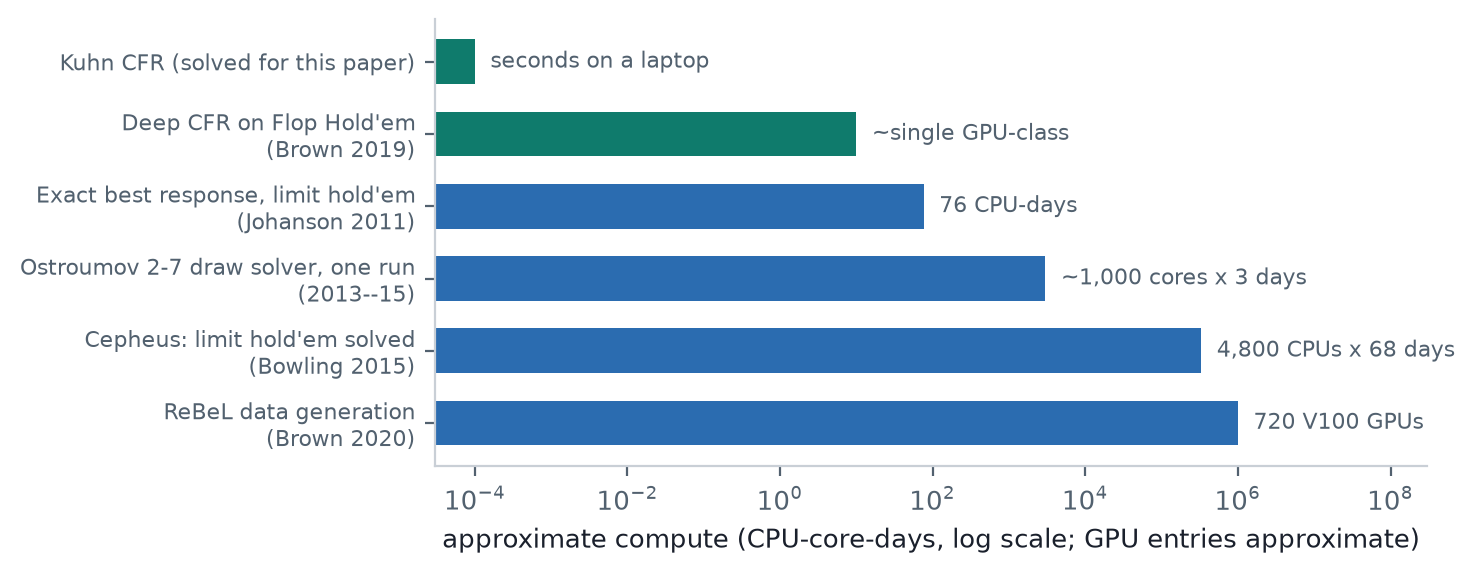
\includegraphics[width=\linewidth]{figures/compute.png}
\caption{Approximate compute of landmark systems, from reported hardware (log scale; order-of-magnitude estimates).}
\label{fig:compute}
\end{figure}

The build itself follows the field's standard validation practice --- prove each layer on a game with a known answer before adding the next --- instantiated for this project as Figure~\ref{fig:ladder}'s ladder. Its logic: Deep CFR has three separately-breakable layers (the CFR core, the Drawmaha rules engine, the networks); climbing one rung at a time means every failure has one suspect. The mini-drawmaha rung earns special emphasis: it is where all three Drawmaha-specific mechanisms (split pot, draw round, face-up draw-1) get proven while exact evaluation is still possible --- and it doubles later as tier 1 of the full evaluation (Section~\ref{sec:evaluation}).

\begin{figure}[t]
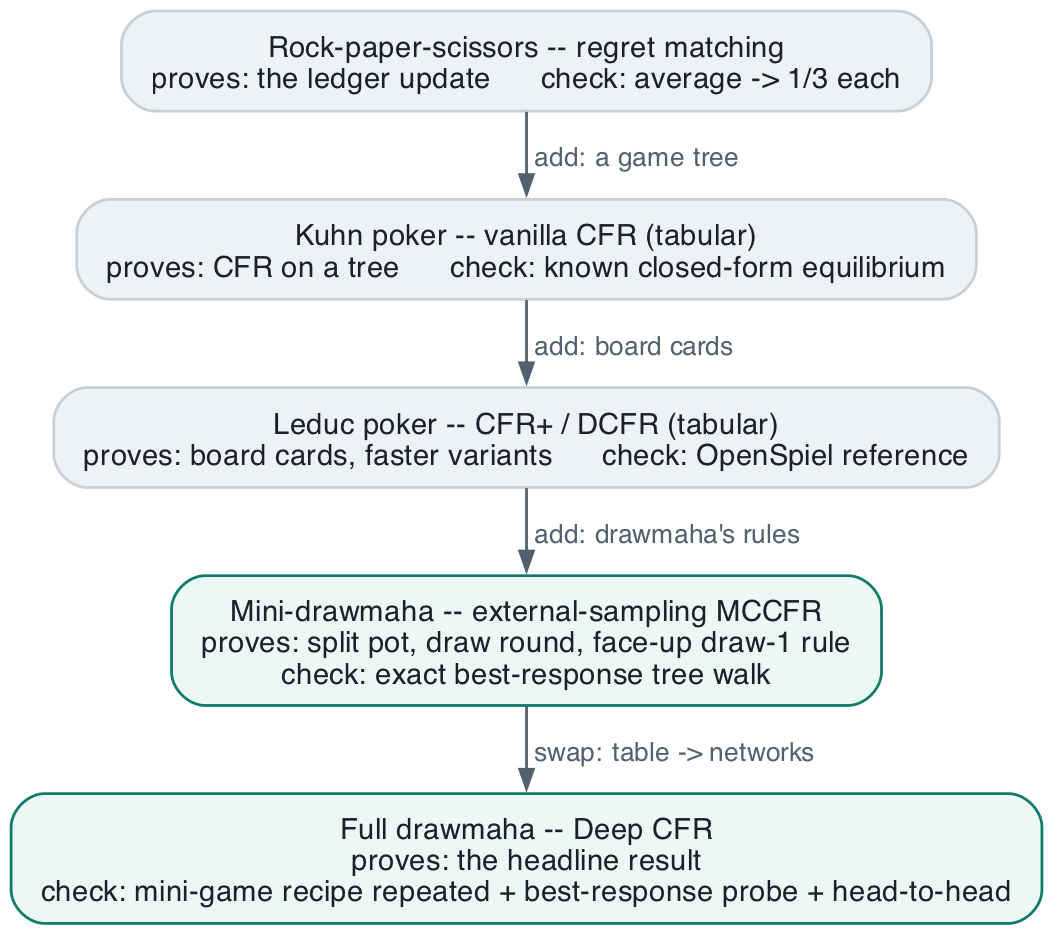
\includegraphics[width=\linewidth]{figures/ladder.png}
\caption{The project's validation ladder: one new layer per rung, a known answer at every rung.}
\label{fig:ladder}
\end{figure}

\section{The decision checklist: every fork this project will actually face}\label{sec:checklist}

\mkey{the checklist}This section is the survey folded into a working document: every design decision the project will meet, bucketed, each with the literature's default and the section that justifies it. Items marked $\circ$ have \emph{no} published answer --- they are the genuinely novel work.

\textbf{A. Game specification (settle before writing the engine)}
\begin{itemize}
\item Rules pinned as in Section~\ref{sec:drawmaha}: HU, pot-limit, \{fold, check/call, pot\} v1 menu as config, 100bb default, one draw post-flop, face-up draw-1 rule, cards-speak split with both-halves tie table written out (including odd-chip handling). Target rake-free play (rake shifts the equilibrium; state the choice).
\item Infoset key contents: own 5 cards (canonicalized) + board + full betting history + \textbf{both players' draw-count histories} + own discard identities + the face-up draw-1 card when present (Sections~\ref{sec:drawmaha},~\ref{sec:precedents}).
\item Scope statements, written once in the README: all guarantees are heads-up (3+ players voids interchangeability and safety, Section~\ref{sec:solving}; the practical stance elsewhere --- Pluribus --- is train HU, accept heuristic multiway play); equilibrium only, no opponent modeling/exploitation (a different literature: restricted Nash response, safe exploitation).
\end{itemize}

\textbf{B. Representation and encoding}
\begin{itemize}
\item Suit-isomorphic canonicalization (134{,}459 classes) keys everything; Waugh-style perfect indexing; expect weaker symmetry postflop (Section~\ref{sec:abstraction}).
\item Card inputs: Deep CFR's summed rank/suit/card embeddings, permutation-invariant over hole cards (Section~\ref{sec:deepcfr}). Betting history: per-slot occurred-flag + pot-fraction features to start.
\item[$\circ$] Discard action head: flat 32-way softmax vs.\ per-card factorized logits --- unexplored; start flat (regret matching over 32 actions is standard), benchmark factorized later.
\item[$\circ$] Draw-signal features: both draw counts, the face-up card, and kept-card identities --- feature design with no citation; validate on mini-drawmaha ablations.
\item Dual evaluator: 5-card perfect hash for the inner hand + Omaha-mode evaluation for the outer; bit-packed ranks; all split logic in terminal payoffs only (Sections~\ref{sec:precedents},~\ref{sec:engineering}).
\end{itemize}

\textbf{C. Training pipeline}
\begin{itemize}
\item The ladder (Fig.~\ref{fig:ladder}): vanilla CFR $\to$ CFR+/DCFR$(1.5,0,2)$ on toys; external-sampling MCCFR with linear weighting on mini-drawmaha; Deep CFR at full scale with the published hyperparameters as anchors (Section~\ref{sec:deepcfr}).
\item SD-CFR-style checkpointing during training, one distilled average-policy net at the end for serving.
\item Escalation valves, in order: VR-MCCFR baselines if sampling noise binds; robust sampling ($k<$ all) if the 32-subset draw node makes traversals slow; ESCHER-style value function if advantage-target variance won't settle; depth-limited resolve at the draw boundary as the accuracy upgrade (Section~\ref{sec:search}).
\item[$\circ$] Mini-drawmaha's exact design (deck size, hand size, streets) --- sized so the exact best-response walk is affordable: shrink the \emph{deck}, not just stacks.
\end{itemize}

\textbf{D. Evaluation protocol (pre-registered, Section~\ref{sec:evaluation})}
\begin{itemize}
\item Units: total-chips-both-halves per hand in bb; compute Drawmaha's own always-fold anchor; per-half EV and scoop-rate diagnostics.
\item Instruments per rung: OpenSpiel-verified exact exploitability (toys); exact walk + Deep-CFR-vs-tabular gap (mini); duplicate-dealt AIVAT head-to-head ladder + trained exploiter, reported as a lower bound (full).
\item Match runner ships with duplicate dealing from day one; every claimed difference carries a bootstrap CI.
\end{itemize}

\textbf{E. Deployment and dashboard}
\begin{itemize}
\item Serving: one forward pass per query on the distilled net; per-node range views computed by batch-evaluating all (canonical) hands with reach probabilities from policy products along the line; memoize visited nodes.
\item Post-processing before display/play: \keyterm{purification}\mdef{purification}{round near-zero action probabilities away before serving; cuts approximation-noise exploitability} and thresholding (Ganzfried \& Sandholm 2012) --- the standard step between ``trained net'' and ``served strategy.''
\item User-typed bet sizes: pseudo-harmonic action translation now; nested re-solving later (Section~\ref{sec:abstraction}).
\item Display bucketing: equity-histogram $k$-means into 8--20 named buckets over canonical classes, filterable by inner/outer hand (the project's chosen UI model).
\end{itemize}

\textbf{F. Open problems worth a writeup of their own}
\begin{itemize}
\item[$\circ$] Belief updates through a hidden discard (marginalizing over which cards were kept given only the count) --- required by any future search layer, written down nowhere.
\item[$\circ$] A 2.6M-hand range representation for value nets (bucketed or factorized) --- the wall between this project and the DeepStack/ReBeL lineage.
\item[$\circ$] LBR adapted to draw games (range tracking through draws, stand-pat heuristics) --- the trained exploiter sidesteps it, but the adaptation would be a contribution.
\end{itemize}

\mnote{Reading order for the build, matched to rungs: Neller \& Lanctot's tutorial (rung 0--1) $\to$ Lanctot 2009 (rung 3's MCCFR) $\to$ Brown 2019 Deep CFR + Steinberger's SD-CFR/PokerRL code (rung 4) $\to$ Lis\'y \& Bowling + Burch AIVAT (evaluation) $\to$ the rest as needed.}Nothing in this list is speculative: every default traces to a cited result, and every $\circ$ is a place where this project, by existing, produces the first data point.

\section{Key takeaways}\label{sec:takeaways}

\begin{enumerate}
\item \textbf{The target is a number.} Solving means driving \emph{exploitability} --- what a perfect adversary wins against you --- toward zero. It is computable exactly on small games, lower-boundable on big ones, and it, not any loss curve, is the project's progress bar.
\item \textbf{One rule, one theorem.} Regret matching (play proportional to positive regret) plus the folk theorem (vanishing average regret $\Rightarrow$ the \emph{average} strategy pair approaches Nash) generate the entire CFR family. The average-vs-current distinction is the field's most common bug and the reason an average-policy network is the deliverable.
\item \textbf{The project's spine is standard and single-GPU-sized.} External-sampling MCCFR with linear weighting, scaled to Deep CFR with the published hyperparameters as anchors, SD-CFR checkpointing during training, one distilled net for serving. Every landmark that needed more compute (Cepheus, ReBeL) is the argument for this choice, not against it.
\item \textbf{Search is the upgrade, not the start.} The DeepStack/ReBeL/GTO-Wizard lineage buys accuracy and custom-spot flexibility at seconds per query --- and its range-vector inputs hit a 2.6M-dimension wall in Drawmaha. Depth-limited resolving at the draw boundary is the one cheap borrowing.
\item \textbf{Plain self-play RL is a trap here, and provably so.} The dynamics orbit; nothing converges; head-to-head wins cannot certify equilibrium quality. Actor--critic earns its place in three supporting roles: the exploiter, the variance baselines, and the comparison chapter.
\item \textbf{Drawmaha's novelties are locatable.} Split pot: terminal payoffs only --- cheap. Hand space: canonicalize (134{,}459 classes) and let networks generalize. Draw round: keep discard identity in the infoset, feed the public counts to the net, and expect the encoding decisions ($\circ$ items, Section~\ref{sec:checklist}) to be the project's first genuinely novel results.
\item \textbf{Validate like the field does.} One new layer per rung, a known answer at every rung, regression constants from Kuhn/Leduc/OpenSpiel, and a pre-registered evaluation protocol --- the practices that separate ``I trained a bot'' from ``I can bound how far it is from equilibrium.''
\end{enumerate}

\vspace{0.4em}
\textbf{Provenance.} Synthesized August 28, 2026 from an eight-lane automated literature sweep (Semantic Scholar, arXiv, and the open web; $\sim$70 sources verified by fetch) plus a completeness audit; lane digests with per-paper notes live in the project repository under \texttt{research/}. Claims the sweep could not verify in-session are flagged in those digests; the cited originals remain ground truth. The Kuhn, RPS, and dynamics figures were computed live by code in \texttt{paper/make\_figures.py}, validated against Kuhn's closed-form game value.

\begingroup
\footnotesize
\begin{thebibliography}{99}
\setlength{\itemsep}{1.5pt}

\bibitem{hart2000} S.~Hart, A.~Mas-Colell. A simple adaptive procedure leading to correlated equilibrium. \emph{Econometrica} 68(5), 2000.
\bibitem{zinkevich2007} M.~Zinkevich, M.~Johanson, M.~Bowling, C.~Piccione. Regret minimization in games with incomplete information. \emph{NIPS}, 2007.
\bibitem{neller2013} T.~Neller, M.~Lanctot. An introduction to counterfactual regret minimization. AAAI Model AI Assignments, 2013. \texttt{modelai.gettysburg.edu/2013/cfr}.
\bibitem{lanctot2009} M.~Lanctot, K.~Waugh, M.~Zinkevich, M.~Bowling. Monte Carlo sampling for regret minimization in extensive games. \emph{NIPS}, 2009.
\bibitem{tammelin2014} O.~Tammelin. Solving large imperfect information games using CFR+. arXiv:1407.5042, 2014.
\bibitem{tammelin2015} O.~Tammelin, N.~Burch, M.~Johanson, M.~Bowling. Solving heads-up limit Texas hold'em. \emph{IJCAI}, 2015.
\bibitem{bowling2015} M.~Bowling, N.~Burch, M.~Johanson, O.~Tammelin. Heads-up limit hold'em poker is solved. \emph{Science} 347(6218), 2015.
\bibitem{brown2019dcfr} N.~Brown, T.~Sandholm. Solving imperfect-information games via discounted regret minimization. \emph{AAAI}, 2019.
\bibitem{brown2015pruning} N.~Brown, T.~Sandholm. Regret-based pruning in extensive-form games. \emph{NIPS}, 2015.
\bibitem{johanson2012pcs} M.~Johanson, N.~Bard, M.~Lanctot, R.~Gibson, M.~Bowling. Efficient Nash equilibrium approximation through Monte Carlo counterfactual regret minimization / public chance sampling. \emph{AAMAS}, 2012.
\bibitem{koller1996} D.~Koller, N.~Megiddo, B.~von~Stengel. Efficient computation of equilibria for extensive two-person games. \emph{Games and Economic Behavior} 14, 1996.
\bibitem{schmid2019vr} M.~Schmid, N.~Burch, M.~Lanctot, M.~Moravcik, R.~Kadlec, M.~Bowling. Variance reduction in Monte Carlo CFR using baselines. \emph{AAAI}, 2019.
\bibitem{gilpin2007} A.~Gilpin, T.~Sandholm. Lossless abstraction of imperfect information games. \emph{Journal of the ACM} 54(5), 2007.
\bibitem{waugh2009} K.~Waugh, D.~Schnizlein, M.~Bowling, D.~Szafron. Abstraction pathologies in extensive games. \emph{AAMAS}, 2009.
\bibitem{waugh2013iso} K.~Waugh. A fast and optimal hand isomorphism algorithm. AAAI Workshop on Computer Poker, 2013.
\bibitem{johanson2013} M.~Johanson, N.~Burch, R.~Valenzano, M.~Bowling. Evaluating state-space abstractions in extensive-form games. \emph{AAMAS}, 2013.
\bibitem{ganzfried2013at} S.~Ganzfried, T.~Sandholm. Action translation in extensive-form games with large action spaces: axioms, paradoxes, and the pseudo-harmonic mapping. \emph{IJCAI}, 2013.
\bibitem{ganzfried2014} S.~Ganzfried, T.~Sandholm. Potential-aware imperfect-recall abstraction with earth mover's distance. \emph{AAAI}, 2014.
\bibitem{ganzfried2012purification} S.~Ganzfried, T.~Sandholm, K.~Waugh. Strategy purification and thresholding: effective non-equilibrium approaches for playing large games. \emph{AAMAS}, 2012.
\bibitem{brown2019deep} N.~Brown, A.~Lerer, S.~Gross, T.~Sandholm. Deep counterfactual regret minimization. \emph{ICML}, 2019.
\bibitem{steinberger2019} E.~Steinberger. Single deep counterfactual regret minimization. arXiv:1901.07621, 2019.
\bibitem{steinberger2020dream} E.~Steinberger, A.~Lerer, N.~Brown. DREAM: deep regret minimization with advantage baselines and model-free learning. arXiv:2006.10410, 2020.
\bibitem{mcaleer2022} S.~McAleer, G.~Farina, M.~Lanctot, T.~Sandholm. ESCHER: eschewing importance sampling in games by computing a history value function to estimate regret. \emph{ICLR}, 2023.
\bibitem{liu2022recfr} W.~Liu, B.~Li, J.~Togelius. Model-free neural counterfactual regret minimization with bootstrap learning. \emph{IEEE Transactions on Games}, 2022.
\bibitem{burch2014} N.~Burch, M.~Johanson, M.~Bowling. Solving imperfect-information games using decomposition. \emph{AAAI}, 2014.
\bibitem{deepstack} M.~Moravcik, M.~Schmid, N.~Burch, V.~Lisy, D.~Morrill, N.~Bard, T.~Davis, K.~Waugh, M.~Johanson, M.~Bowling. DeepStack: expert-level artificial intelligence in heads-up no-limit poker. \emph{Science} 356(6337), 2017.
\bibitem{libratus} N.~Brown, T.~Sandholm. Superhuman AI for heads-up no-limit poker: Libratus beats top professionals. \emph{Science} 359(6374), 2018. (Nested subgame solving: \emph{NIPS} 2017.)
\bibitem{brown2018dls} N.~Brown, T.~Sandholm, B.~Amos. Depth-limited solving for imperfect-information games. \emph{NeurIPS}, 2018.
\bibitem{pluribus} N.~Brown, T.~Sandholm. Superhuman AI for multiplayer poker. \emph{Science} 365(6456), 2019.
\bibitem{rebel} N.~Brown, A.~Bakhtin, A.~Lerer, Q.~Gong. Combining deep reinforcement learning and search for imperfect-information games. \emph{NeurIPS}, 2020.
\bibitem{sog} M.~Schmid et al. Student of Games: a unified learning algorithm for both perfect and imperfect information games. \emph{Science Advances} 9, 2023.
\bibitem{gtowizardai} GTO Wizard. GTO Wizard AI explained; How solvers work; How GTO Wizard solved PLO. Company engineering blog, 2023--2026 (vendor claims, no peer review). \texttt{blog.gtowizard.com}.
\bibitem{perolat2020} J.~Perolat, R.~Munos, J.-B.~Lespiau, et al. From Poincar\'e recurrence to convergence in imperfect information games: finding equilibrium via regularization. \emph{ICML}, 2021.
\bibitem{alphazero} D.~Silver et al. Mastering chess and shogi by self-play with a general reinforcement learning algorithm. arXiv:1712.01815, 2017; \emph{Science} 362, 2018.
\bibitem{nfsp} J.~Heinrich, D.~Silver. Deep reinforcement learning from self-play in imperfect-information games. arXiv:1603.01121, 2016.
\bibitem{psro} M.~Lanctot, V.~Zambaldi, A.~Gruslys, et al. A unified game-theoretic approach to multiagent reinforcement learning. \emph{NeurIPS}, 2017.
\bibitem{deepnash} J.~Perolat, B.~De~Vylder, D.~Hennes, et al. Mastering the game of Stratego with model-free multiagent reinforcement learning. \emph{Science} 378, 2022.
\bibitem{mmd} S.~Sokota, R.~D'Orazio, J.Z.~Kolter, N.~Loizou, M.~Lanctot, I.~Mitliagkas, N.~Brown, C.~Kroer. A unified approach to reinforcement learning, quantal response equilibria, and two-player zero-sum games. \emph{ICLR}, 2023.
\bibitem{alphaholdem} E.~Zhao, R.~Yan, J.~Li, K.~Li, J.~Xing. AlphaHoldem: high-performance artificial intelligence for heads-up no-limit poker via end-to-end reinforcement learning. \emph{AAAI}, 2022.
\bibitem{timbers2022} F.~Timbers, N.~Bard, E.~Lockhart, M.~Lanctot, M.~Schmid, N.~Burch, J.~Schrittwieser, T.~Hubert, M.~Bowling. Approximate exploitability: learning a best response in large games. \emph{IJCAI}, 2022.
\bibitem{vrpo} Z.~Fan, G.~Farina. GAE falls short in imperfect-information self-play reinforcement learning. arXiv preprint, 2026 (unreviewed).
\bibitem{johanson2011} M.~Johanson, K.~Waugh, M.~Bowling, M.~Zinkevich. Accelerating best response calculation in large extensive games. \emph{IJCAI}, 2011.
\bibitem{lbr} V.~Lisy, M.~Bowling. Equilibrium approximation quality of current no-limit poker bots (local best response). AAAI Workshop on Computer Poker, 2017.
\bibitem{aivat} N.~Burch, M.~Schmid, M.~Moravcik, M.~Bowling. AIVAT: a new variance reduction technique for agent evaluation in imperfect information games. \emph{AAAI}, 2018.
\bibitem{acpc} N.~Bard, J.~Hawkin, J.~Rubin, M.~Zinkevich. The annual computer poker competition. \emph{AI Magazine} 34(2), 2013.
\bibitem{ostroumov} O.~Ostroumov. How I made my first million: story of Draw Solver (2-7 triple draw / badugi). First-person engineering account, GipsyTeam/Medium, 2025 (practitioner source).
\bibitem{ho2015} K.~Ho. A no-limit Omaha hi-lo poker jam/fold endgame equilibrium. Master's thesis, Harvard Extension School, 2015.
\bibitem{pokercnn} N.~Yakovenko, L.~Cao, C.~Raffel, J.~Fan. Poker-CNN: a pattern learning strategy for making draws and bets in poker games. \emph{AAAI}, 2016.
\bibitem{zadeh} N.~Zadeh. Computation of optimal poker strategies. \emph{Operations Research} 25(4), 1977.
\bibitem{ginrummy} B.~Goldstein, J.-P.~Astudillo~Guerra, E.~Haigh, B.~Cruz~Ulloa, J.~Blum. Extracting learned discard and knocking strategies from a gin rummy bot. \emph{AAAI/EAAI}, 2021.
\bibitem{openspiel} M.~Lanctot, E.~Lockhart, et al. OpenSpiel: a framework for reinforcement learning in games. arXiv:1908.09453, 2019.
\bibitem{pokerrl} E.~Steinberger. PokerRL (with Deep-CFR/SD-CFR reference implementations). \texttt{github.com/EricSteinberger/PokerRL}, 2019.
\bibitem{rlcard} D.~Zha, K.-H.~Lai, Y.~Cao, S.~Huang, R.~Wei, J.~Guo, X.~Hu. RLCard: a toolkit for reinforcement learning in card games. AAAI-20 Workshop, 2019.
\bibitem{pokerkit} J.~Kim. PokerKit: a comprehensive Python library for fine-grained multi-variant poker game simulations. \emph{IEEE Transactions on Games}, 2023.
\bibitem{cactuskev} K.~Suffecool (Cactus Kev); P.~Senzee; and descendants (OMPEval, PokerHandEvaluator). Fast 5-card hand evaluation via 7{,}462 equivalence classes and perfect hashing. Community engineering lineage, 2006--. \texttt{suffe.cool/poker/evaluator.html}.

\end{thebibliography}
\endgroup


\end{document}
